\documentclass[oneside, doctor]{NJUPT-Thesis_professional-grd}
%oneside选项表示单页打印,twoside选项表示双页打印. 默认单面 oneside。
%建议最终论文打印时采用双页打印

%专业型硕士选择NJUPT-Thesis_professional-grd，盲审将NJUPT-Thesis_professional-grd替换为NJUPT-Thesis_professional-grd_Blind

\raggedbottom


\begin{document}


\institutenumber{10293}
\confidential{}%这里输入密级
\title{}%这里输入论文题目
\studentnumber{}%这里输入学号
\author{}%这里输入姓名
\advisor{}%这里输入导师
\major{}%这里输入专业学位类别
%\institute{通信与信息工程学院}
\interest{}%这里输入类型
%\school{南京邮电大学}
\degree{****}%这里输入专业（领域）
\defenddate{}%这里输入论文提交日期

% 英文封面内容
\englishtitle{*****************************\\
	***********************}%这里输入论文英文标题
\englishauthor{******}%这里输入作者英文名字
\englishadvisor{Prof. ******}%这里输入导师英文名字
\englishdate{**~****}%这里输入论文提交日期如：April  2018

% 首页封面绘制
% \maketitle

% 中文标题页绘制
\makeInfo

% 英文标题页绘制
%\makeEnglishInfo

% 论文原创性声明和使用授权声明绘制
%\makeDeclareOriginal

%%%%%%%%%%%%前置部分%%%%%%%%%%%%
\frontmatter

% 摘要
\begin{abstract}
  离线强化学习从行为策略收集的静态数据集中学习策略，避免了在线交互的高昂成本与安全风险，在医疗诊断、自动驾驶、机器人控制等实际应用场景中具有重要价值。然而，由于行为策略通常是次优的，且离线数据集覆盖范围有限，分布偏移问题成为制约离线强化学习发展的核心挑战：当策略访问离线数据未覆盖的状态-动作对时，价值函数的估计将产生外推误差，进而导致策略性能退化。针对这一问题，本文以不确定性量化为核心手段展开系统研究：首先解决纯离线设定下的保守策略优化问题；在此基础上，针对离线数据覆盖边界对策略性能的根本性约束，进一步研究如何通过定向探索突破数据边界，形成从离线保守优化到在线高效微调的完整技术方案。

  在保守策略优化方面，本文提出基于自适应不确定性度量的离线强化学习算法。针对现有基于模型方法仅考虑状态转移不确定性、采用静态惩罚系数的局限，引入累积状态不确定性度量和自适应动态权重机制。累积状态不确定性通过递推公式综合考虑历史不确定性的累积效应，使智能体能够更全面地评估决策风险；自适应动态权重机制基于Sigmoid函数动态调节惩罚强度，实现探索与保守的自适应平衡。理论分析证明累积不确定性的单调性和自适应权重的优越性。实验结果表明，该方法在D4RL MuJoCo基准测试集上显著优于MOPO等基线方法。

  上述纯离线方法的策略性能仍受限于离线数据的覆盖范围。为突破这一根本性约束，本文进一步提出基于定向探索模型的离线到在线强化学习算法。该方法将不确定性信息从“惩罚信号”转变为“探索引导信号”：在离线阶段通过集成模型进行保守策略优化，在在线阶段显式引导策略探索高不确定性且高价值的区域。提出双重不确定性估计方法区分偶然不确定性和认知不确定性，设计动态权重自适应机制平滑过渡探索与利用。理论分析证明定向探索策略相比均匀采样具有更优的收敛速率。实验结果表明，该方法仅需50k步在线交互即可显著优于现有基线方法。

  \keywords{离线强化学习，不确定性估计，分布偏移，定向探索，离线到在线强化学习}

\end{abstract}

















\begin{englishabstract}

  Offline reinforcement learning enables policy learning from pre-collected static datasets, avoiding the high costs and safety risks of online interactions. This approach holds significant practical value in domains such as medical diagnosis, autonomous driving, and robotic control. However, since behavioral strategies are generally suboptimal and offline datasets have limited coverage, the core challenge hindering offline reinforcement learning: when the learned policy visits state-action pairs not covered by offline data, value function estimation produces extrapolation errors, leading to performance degradation. To address this problem, this thesis systematically studies uncertainty quantification: first solving the conservative policy optimization problem in purely offline settings; then, to overcome the fundamental constraint that offline data boundaries impose on policy performance, investigating how directed exploration can transcend these boundaries, forming a complete technical solution from offline conservative optimization to efficient online fine-tuning.

  In conservative policy optimization, an offline reinforcement learning algorithm based on adaptive uncertainty measurement is proposed. To address the limitations of existing model-based methods that only consider state transition uncertainty and employ static penalty coefficients, cumulative state uncertainty measurement and an adaptive dynamic weight mechanism are introduced. The cumulative state uncertainty comprehensively accounts for accumulated historical uncertainty through a recursive formula, enabling more thorough risk assessment. The adaptive dynamic weight mechanism based on Sigmoid function dynamically adjusts penalty strength to achieve better exploration-conservatism balance. Theoretical analysis proves the monotonicity of cumulative uncertainty and the superiority of adaptive weights. Experiments demonstrate significant improvements over MOPO on the D4RL MuJoCo benchmark.

  The above purely offline method's policy performance remains constrained by offline data coverage. To break through this fundamental limitation, an offline-to-online reinforcement learning algorithm based on directed exploration is further proposed. This method transforms uncertainty information from a "penalty signal" to an "exploration guide": during offline learning, conservative policy optimization is performed via ensemble models; during online learning, the policy is explicitly guided to explore high-uncertainty, high-value regions. A dual uncertainty estimation method distinguishes aleatoric and epistemic uncertainty, with a dynamic weight adaptation mechanism smoothing the transition between exploration and exploitation. Theoretical analysis proves superior convergence rates compared to uniform sampling. Experiments show significant improvements over baselines with only 50k online interaction steps.

  \englishkeywords{offline reinforcement learning, uncertainty estimation, distribution shift, directed exploration, offline-to-online reinforcement learning}

\end{englishabstract}


% 加入目录
\tableofcontents

%加入图、表索引(同时取消图表索引中章之间的垂直间隔)

\let\origaddvspace\addvspace
\renewcommand{\addvspace}[1]{}
\listoffigures
\addcontentsline{toc}{chapter}{插图索引}
\listoftables
\addcontentsline{toc}{chapter}{表格索引}
\renewcommand{\addvspace}[1]{\origaddvspace{#1}}

 % 主要符号对照表
% \input{chapters/denotation}
% % 缩略词列表
% \input{chapters/abbreviation}

% 专用术语注释表
\begin{denoabbre}

  \noindent {\bf{符号说明：}} \vspace{-13pt} \\

  \begin{supertabular}{p{4cm}p{9cm}}
    {\textbf{\heiti{符号}}}  &  {\textbf{\heiti{表示含义}}}    \\
    $\mathcal{S}$  &  状态空间 \\
    $\mathcal{A}$  &  动作空间 \\
    $T(s'\mid s,a)$  &  状态转移概率函数 \\
    $r(s,a)$  &  奖励函数 \\
    $\mu_0$  &  初始状态分布 \\
    $\gamma$  &  折扣因子 \\
    $\pi(a\mid s)$  &  策略（在状态$s$下选择动作$a$的概率） \\
    $V^\pi(s)$  &  状态价值函数 \\
    $Q^\pi(s,a)$  &  动作价值函数 \\
    $\rho^\pi(s,a)$  &  折扣状态-动作访问分布 \\
    $\mathcal{D}_{off}$  &  离线数据集（由行为策略预先收集） \\
    $\mathcal{D}_{on}$  &  在线交互数据集（微调阶段采集） \\
    $\mathcal{D}_{model}$  &  模型生成的虚拟轨迹数据集 \\
    $\hat{T}_\theta(s',r\mid s,a)$  &  学习得到的概率转移模型 \\
    $\mu_\theta(s,a)$  &  转移模型预测的均值（含$s'$与$r$） \\
    $\Sigma_\theta(s,a)$  &  转移模型预测的协方差/方差（不确定性来源之一） \\
    $u_{trans}(s,a)$  &  单步状态转移不确定性度量 \\
    $u(s)$  &  累积状态不确定性（沿轨迹传播与累积） \\
    $u_\phi(s)$  &  累积不确定性预测网络的输出 \\
    $\omega$  &  累积不确定性折扣因子 \\
    $\tilde{r}(s,a)$  &  引入不确定性惩罚后的重塑奖励 \\
    $\lambda_0$  &  基础惩罚系数（自适应权重的上界） \\
    $\lambda_k$  &  第$k$轮训练的自适应惩罚权重 \\
    $K_0$  &  自适应权重的转折点（Sigmoid中心） \\
    $\alpha$  &  状态不确定性与转移不确定性的平衡系数（第3章） \\
    $\alpha_{ent}$  &  熵温度参数（SAC中平衡探索/利用） \\
    $\text{DisVar}(s,a)$  &  集成模型均值分歧度（认知不确定性度量） \\
    $u_{on}(s,a)$  &  在线阶段综合不确定性（偶然+认知） \\
    $c$  &  在线阶段不确定性引导权重（定向探索） \\
    $c_0$  &  在线阶段初始探索权重 \\
    $k_0,\,\nu$  &  探索权重衰减中心与衰减速率参数 \\
    $N$  &  集成模型成员数量 \\
    $B$  &  在线交互预算（可用交互步数上限） \\
    $\beta_t$  &  混合重放中在线数据采样比例 \\


  \end{supertabular}  \vspace{50pt}


  \noindent {\bf{缩略词说明：}} \vspace{-13pt} \\

  \begin{supertabular}{p{2.5cm}p{8.5cm}p{8cm}}
    {\textbf{\heiti{缩写}}}  &  {\textbf{\heiti{英文全称}}}  &   {\textbf{\heiti{中文译名}}}   \\
    RL   &  Reinforcement Learning  &  强化学习 \\
    Offline RL   &  Offline Reinforcement Learning  &  离线强化学习 \\
    O2O RL   &  Offline-to-Online Reinforcement Learning  &  离线到在线强化学习 \\
    MDP   &  Markov Decision Process  &  马尔可夫决策过程 \\
    SAC   &  Soft Actor-Critic  &  软演员-评论家算法 \\
    TD3   &  Twin Delayed Deep Deterministic Policy Gradient  &  双延迟深度确定性策略梯度 \\
    BC   &  Behavior Cloning  &  行为克隆 \\
    BCQ   &  Batch-Constrained Q-learning  &  批约束Q学习 \\
    CQL   &  Conservative Q-Learning  &  保守Q学习 \\
    IQL   &  Implicit Q-Learning  &  隐式Q学习 \\
    MOPO   &  Model-based Offline Policy Optimization  &  基于模型的离线策略优化 \\
    MOReL   &  Model-Based Reinforcement Learning  &  基于模型的强化学习方法（悲观MDP路线） \\
    COMBO   &  Conservative Offline Model-Based Policy Optimization  &  保守的离线基于模型策略优化 \\
    AWAC   &  Advantage-Weighted Actor-Critic  &  优势加权演员-评论家 \\
    PETS   &  Probabilistic Ensembles with Trajectory Sampling  &  概率集成与轨迹采样 \\
    MBPO   &  Model-Based Policy Optimization  &  基于模型的策略优化 \\
    D4RL   &  Datasets for Deep Data-Driven Reinforcement Learning  &  深度数据驱动强化学习数据集基准 \\
    MuJoCo   &  Multi-Joint dynamics with Contact  &  多关节动力学仿真平台 \\
    OOD   &  Out-Of-Distribution  &  分布外（样本/动作） \\
    KL   &  Kullback--Leibler Divergence  &  KL散度 \\
    MMD   &  Maximum Mean Discrepancy  &  最大均值差异 \\
    CVAE   &  Conditional Variational Autoencoder  &  条件变分自编码器 \\
    t-SNE   &  t-distributed Stochastic Neighbor Embedding  &  t分布随机邻域嵌入（可视化） \\


  \end{supertabular}

\end{denoabbre}


%本部分内容非强制性要求，如果论文中所用符号不多，可以省略《专用术语注释表》。


%%%%%%%%%%%%正文主体部分% %%%%%%%%%%%
\mainmatter
% 各章正文内容
\chapter{绪论}\label{Chap:chap1}


\section{研究背景与意义}\label{Sec1.1}

强化学习（Reinforcement Learning, RL）是一种实现机器自主决策的人工智能范式，智能体通过与环境的持续交互学习最优策略，以最大化长期累积回报\cite{Levine2020OfflineRL}。自深度强化学习在围棋\cite{Silver2016AlphaGo}等领域取得突破以来，学术界与工业界持续将其应用拓展至更复杂的真实场景。近年来，强化学习在机器人控制\cite{Johannink2019Residual}领域积累了丰富经验，并随着DeepSeek-R1\cite{DeepSeekAI2025R1}在推理任务中的成功应用，开始广泛用于大语言模型的对齐与微调。

在线强化学习框架中，智能体直接与环境交互，通过试错优化行为策略。该方法具备良好的适应性，能够根据环境反馈及时调整策略，但需要大量交互样本。在医疗诊断\cite{Gottesman2019Healthcare}、自动驾驶\cite{Kiran2022Driving}等数据采集成本高昂或存在安全约束的场景中，频繁的在线试错既不经济也存在风险，限制了在线强化学习的实际部署。

离线强化学习提供了一种替代方案：从预先收集的静态数据集中学习策略，避免在线交互的成本与风险。该范式依赖行为策略采集的历史数据，训练开销较小。然而，行为策略通常是次优的，且存在分布偏移问题\cite{Fujimoto2019BCQ}——训练数据分布与目标策略访问的状态-动作分布存在差异，导致价值函数对分布外动作的估计不准确。由于离线学习无法获得环境反馈修正估计误差，累积误差会引发对分布外动作价值的过高估计，产生外推误差\cite{Liu2020Provably}。如何从有限且可能存在偏差的数据中学习泛化能力良好的策略，是离线强化学习的核心挑战。

离线到在线强化学习结合了两种范式的优势：先在离线数据上预训练策略，再通过有限的在线交互进行微调，既利用了历史数据降低样本需求，又通过在线反馈提升策略性能。

当前离线到在线方法多采用无模型框架，侧重于离线与在线数据的融合策略，如平衡重放、优先级采样等。无模型方法的样本效率受限，难以充分挖掘大规模离线数据集的价值。本文研究基于不确定性探索模型的离线到在线强化学习算法，将优化重点置于环境动力学模型：利用离线策略与环境交互获取的在线数据优化状态转移模型，构建更准确且覆盖分布外区域的环境模型，进而完成策略更新。该方法以模型生成数据替代频繁的环境交互，在线开销较小，数据利用效率较高。

引入不确定性量化机制后，该方法在离线阶段可识别数据集中的高不确定性区域，对这些区域采取保守的策略更新；在线阶段则优先探索不确定性较高的状态-动作对，以较小的交互代价获取策略未覆盖区域的新数据。这种不确定性引导的探索机制提升了模型对环境变化的适应能力。

该算法适用于需要充分利用历史数据、同时在线探索受限的场景，如自动驾驶、金融决策、医疗优化等。基于模型的框架通过数据生成减少对在线交互的依赖，不确定性引导的探索策略提升了在线微调的样本效率，在控制在线成本的同时实现策略性能的持续提升。


\section{国内外研究现状}\label{Sec1.2}

强化学习在决策优化领域的应用日趋成熟，学术界与工业界均取得了阶段性进展。在大语言模型领域，DeepSeek发布的R1系列模型\cite{DeepSeekAI2025R1}通过纯强化学习范式激发模型的复杂推理能力，验证了强化学习在语言模型对齐中的有效性；ByteDance等团队提出的DAPO算法\cite{Yu2025DAPO}开源了大规模语言模型强化学习训练系统，在Qwen2.5-32B基座模型上实现了可复现的推理能力训练。在具身智能领域，Google DeepMind研发的RT-2模型\cite{Brohan2023RT2}将视觉-语言预训练知识迁移至机器人控制，提升了机器人在真实环境中的语义理解与操作泛化能力。在离线强化学习理论研究方面，王雪松等\cite{Wang2024Representation}系统梳理了基于表征学习的离线强化学习方法，分析了特征解耦对策略迁移能力的增强作用。

上述进展表明强化学习在大模型对齐、表征学习、复杂场景适配等方向取得了实质性成果，但也对离线到在线强化学习技术提出了更高要求。当前该领域仍面临若干技术挑战：离线阶段基于固定数据集训练的策略在在线环境中因数据分布差异易产生性能衰减，而在线微调过程中又可能丢失离线阶段习得的知识，现有方案通过动态策略调整、重要性加权等机制尝试平衡两者，但需针对具体任务分析数据分布特性并设计回放机制，开发成本较高。此外，探索-利用权衡是强化学习的固有难题，离线到在线的两阶段模式进一步放大了这一矛盾——离线阶段需保持策略保守性以规避数据偏差风险，在线阶段又需探索未知区域以适配环境变化，两阶段对探索强度的需求相反，RT-2模型虽提升了泛化能力，但未形成适配两阶段特性的动态探索机制。在数据利用效率方面，离线数据集的知识常未被充分利用，策略在微调阶段易丢失预训练知识；在线交互虽能获取环境反馈，但频繁访问环境会削弱离线学习低成本的优势，如何在提升数据利用率的同时控制在线开销，是该领域亟待解决的问题。

上述挑战推动了基于不确定性探索等技术方案的研究，也是本文的研究出发点。


\section{研究内容与主要工作}\label{Sec1.3}
% TODO: 根据论文实际内容补充


\section{文章结构安排}\label{Sec1.4}
% TODO: 根据论文实际章节安排补充































\chapter{理论基础与相关工作}\label{Chap:chap2}

本章首先介绍强化学习的理论基础，建立本文所需的数学框架；随后对离线强化学习、离线到在线强化学习领域的相关工作进行系统综述，分析现有方法的发展脉络、核心优势与局限，阐明本文研究动机。


\section{理论基础}\label{Sec2.1}


\subsection{马尔可夫决策过程}\label{Sec2.1.1}

强化学习问题通常建模为马尔可夫决策过程（Markov Decision Process, MDP）\cite{Sutton2018RLBook}。MDP由六元组$M = (\mathcal{S}, \mathcal{A}, T, r, \mu_0, \gamma)$定义，其中$\mathcal{S}$表示状态空间，$\mathcal{A}$表示动作空间，$r(s,a)$为奖励函数，$T(s'|s,a)$为状态转移函数，$\mu_0$为初始状态分布，$\gamma \in (0,1)$为折扣因子。

状态价值函数$V_M^\pi(s)$表示在MDP $M$中，从状态$s$出发遵循策略$\pi$所能获得的期望折扣回报：
\begin{equation}\label{Eq:Chap2_value_function}
	V_M^\pi(s) = \mathbb{E}_{\pi, M}\left[\sum_{t=0}^{\infty} \gamma^t r(s_t, a_t)\right]
\end{equation}

期望折扣回报$\eta_M^\pi$可通过初始状态分布$\mu_0$下状态价值函数的期望得到：
\begin{equation}\label{Eq:Chap2_expected_return}
	\eta_M^\pi = \mathbb{E}_{s \sim \mu_0}[V_M^\pi(s)]
\end{equation}

MDP的目标是找到最大化$\eta_M^\pi$的最优策略。

动作价值函数$Q_M^\pi(s,a)$表示在状态$s$执行动作$a$后，遵循策略$\pi$所能获得的期望折扣回报。设$\rho_M^\pi(s,a)$为策略$\pi$下的（非归一化）折扣状态-动作访问分布：
\begin{equation}\label{Eq:Chap2_visit_distribution}
	\rho_M^\pi(s,a) = \pi(a|s) \sum_{t=0}^{\infty} \gamma^t P(s_t = s | \pi, M)
\end{equation}

其中$P(s_t=s | \pi, M)$表示在MDP $M$中遵循策略$\pi$于时刻$t$到达状态$s$的概率。期望折扣回报可表示为：
\begin{equation}\label{Eq:Chap2_expected_return_rho}
	\eta_M^\pi = \mathbb{E}_{\rho_M^\pi} \left[ r(s, a) \right]
\end{equation}

归一化状态-动作访问分布定义为$\tilde{\rho}_M^\pi(s,a) = (1 - \gamma) \cdot \rho_M^\pi(s,a)$。


\subsection{基于模型的离线强化学习框架}\label{Sec2.1.2}

在离线强化学习中，智能体仅能访问由行为策略$\pi_D$采集的静态数据集$\mathcal{D}_{off} = \{(s_i, a_i, s_i', r_i)\}_{i=1}^N$，而无法与环境交互。为优化策略，基于模型的离线强化学习首先通过监督学习构建转移模型$\hat{T}_{\theta}(s', r|s, a)$，该模型根据当前状态$s$和动作$a$预测下一状态$s'$和奖励$r$。

转移模型通常表示为高斯分布$\hat{T}_{\theta}(s', r|s, a) = \mathcal{N}(\mu_{\theta}(s, a), \Sigma_{\theta}(s, a))$，其中$\mu_{\theta}(s, a)$为分布均值，$\Sigma_{\theta}(s, a)$为方差。策略可通过与该监督学习得到的转移模型交互进行优化。基于模型的方法在数据采集困难时具有更高的样本效率，但真实环境与监督学习得到的转移模型之间的差异会累积外推误差，导致分布偏移问题。因此，减少分布外数据的过估计对于基于模型的离线强化学习至关重要。


\subsection{集成模型与不确定性估计}\label{Sec2.1.3}

集成方法通过训练多个独立模型，利用模型间预测的分歧度估计不确定性\cite{Lakshminarayanan2017Ensemble}。设训练$N$个模型$\{f_1, \ldots, f_N\}$，预测不确定性可通过集成预测的方差估计。

强化学习中的不确定性可分为两类：\textbf{认知不确定性（Epistemic Uncertainty）}源于知识的缺乏，可通过收集更多数据降低；\textbf{偶然不确定性（Aleatoric Uncertainty）}源于环境固有的随机性，无法通过更多数据消除。对于离线到在线强化学习，认知不确定性尤为重要：高认知不确定性区域对应离线数据覆盖不足的区域，是在线探索应优先关注的目标。

在基于模型的强化学习中，集成动力学模型的每个成员输出高斯分布，其预测方差$\Sigma_\phi^i(s,a)$反映偶然不确定性。为进一步捕捉认知不确定性，可利用集成模型均值预测的分歧度：
\begin{equation}\label{Eq:Chap2_disvar}
	\text{DisVar}(s,a) = \frac{1}{d}\sum_{j=1}^d \text{Var}_{i=1,\ldots,N}[\mu_{\phi,j}^i(s,a)]
\end{equation}

其中$d$为预测向量维度，$\text{Var}_i$表示集成模型间的方差。本文将在算法设计中结合两类不确定性，实现更有效的在线探索。


\section{离线强化学习相关工作}\label{Sec2.2}

离线强化学习（Offline Reinforcement Learning）旨在仅利用预先收集的静态数据集学习策略，而不与环境进行交互\cite{Levine2020OfflineRL}。该范式在机器人控制\cite{Johannink2019Residual}、自动驾驶\cite{Kiran2022Driving}、医疗决策\cite{Gottesman2019Healthcare}等探索成本高昂或存在安全风险的领域具有重要应用价值。离线强化学习面临的核心挑战是\textbf{分布偏移（Distribution Shift）}问题\cite{Fujimoto2019BCQ}：当学习策略与行为策略差异较大时，策略可能访问离线数据集未覆盖的状态-动作对，导致价值函数的外推误差（Extrapolation Error）\cite{Liu2020Provably}。根据是否学习环境模型，离线强化学习方法可分为无模型方法和基于模型方法两大类。


\subsection{无模型离线强化学习}\label{Sec2.2.1}

无模型离线强化学习直接利用离线数据优化策略，其核心思想是在价值函数或策略中引入保守性约束，避免对分布外动作的过估计\cite{Wu2019BRAC,Xu2022PGIS,Kumar2019BEAR,Lyu2022MCQ,Kostrikov2022IQL}。

\textbf{策略约束方法}是该领域的早期探索方向。BCQ\cite{Fujimoto2019BCQ}首次系统分析了离线强化学习中的外推误差问题，提出通过生成模型约束策略仅在行为策略支撑集内选择动作。BRAC\cite{Wu2019BRAC}进一步系统研究了策略正则化方法，通过KL散度或MMD度量约束学习策略与行为策略的距离。TD3+BC\cite{Fujimoto2021TD3BC}则采用更简洁的行为克隆正则项，以极简方式实现策略约束。策略约束方法的\textbf{优势}在于直观有效地避免分布外动作，\textbf{局限}在于策略改进空间受行为策略质量限制，难以超越数据集中最优轨迹的性能。

\textbf{价值正则化方法}从价值函数角度抑制过估计。CQL\cite{Kumar2020CQL}引入正则项学习保守的Q值下界，通过推低分布外动作的Q值、推高数据集内动作的Q值实现保守估计。MCQ\cite{Lyu2022MCQ}在CQL基础上引入更温和的保守约束，避免过度惩罚。IQL\cite{Kostrikov2022IQL}采用期望回归学习价值函数，通过非对称损失函数隐式逼近最优Q值，完全避免对分布外动作的显式查询。价值正则化方法的\textbf{优势}在于无需显式建模行为策略，理论保证更为完善；\textbf{局限}在于保守性可能过强，导致策略性能低于数据集中最优轨迹。

无模型方法的共同\textbf{局限}在于无法生成新的数据样本，样本效率较低，且保守性约束可能限制策略的潜在性能。


\subsection{基于模型的离线强化学习}\label{Sec2.2.2}

基于模型的离线强化学习首先从离线数据学习环境转移模型，再通过与模型交互优化策略\cite{Janner2019MBPO,Yu2020MOPO,Wang2021MORI,Lu2024SER}。该类方法的\textbf{优势}在于可利用模型生成额外数据，提升样本效率。然而，模型在分布外区域的预测可能产生外推误差\cite{Liu2020Provably}，且误差会随rollout步数累积，导致性能退化。因此，基于模型的方法需在探索分布外数据与保持保守性之间取得平衡。

\textbf{不确定性惩罚方法}是该领域的主流范式。MOPO\cite{Yu2020MOPO}提出通过集成模型估计不确定性，对模型预测的奖励施加不确定性惩罚，约束策略在低不确定性区域内优化。该方法的\textbf{优势}在于提供了理论保证的性能下界；\textbf{局限}在于惩罚系数需要针对不同任务调整，且过强的惩罚可能限制策略性能。

\textbf{悲观MDP方法}从另一角度实现保守性。MOReL\cite{Kidambi2020MOReL}构建悲观MDP：当模型不确定性超过阈值时，将状态转移至吸收状态并给予低奖励，从而约束策略在高置信区域内优化。RAMBO\cite{Rigter2022RAMBO}通过对抗训练学习悲观模型，无需显式设定不确定性阈值。该类方法的\textbf{优势}在于提供更强的安全保证；\textbf{局限}在于悲观性可能过强，导致策略过于保守。

\textbf{保守价值估计方法}将无模型方法的保守性与模型数据结合。COMBO\cite{Yu2021COMBO}在模型生成数据上采用CQL的保守估计，在真实数据上进行标准学习，兼顾数据效率与保守性。该方法的\textbf{优势}在于结合了两类方法的优点；\textbf{局限}在于仍受CQL保守性的限制。

近年来，研究者开始引入\textbf{扩散模型}提升转移模型的表达能力\cite{Sun2024Conformal,Zhou2024Diffusion}，能够更好地捕捉多模态转移分布。

尽管上述方法在一定程度上缓解了外推误差，但核心局限在于：\textbf{不确定性信息仅用于惩罚高不确定性区域，而非主动引导策略补充这些区域的数据}。这导致模型在分布外区域的泛化能力始终受限，难以充分评估和补充分布外数据。


\section{离线到在线强化学习相关工作}\label{Sec2.3}

离线到在线强化学习（Offline-to-Online RL）旨在结合离线学习与在线学习的优势：先在离线数据集上预训练策略，再通过有限的在线交互进行微调，提升策略性能。该范式的核心挑战在于\textbf{灾难性遗忘（Catastrophic Forgetting）}：预训练策略在在线微调初期可能出现性能骤降，原因是策略约束的放松导致对分布外状态的访问增加，而价值函数对这些状态的估计不可靠。


\subsection{保守性调节方法}\label{Sec2.3.1}

当前主流方法通过在离线阶段采用保守算法、在线阶段逐步放松约束来平滑过渡\cite{Zhao2023E2O}。AWAC\cite{Nair2020AWAC}通过优势加权回归隐式约束策略接近数据集中的高质量动作，自然适配离线到在线转换。PEX\cite{Zhang2023PEX}维护离线策略与在线策略的混合，根据在线性能动态调整混合权重，在安全性与灵活性之间取得平衡。Cal-QL\cite{Nakamoto2024CalQL}发现离线预训练的Q值可能过于保守或乐观，提出通过校准Q值确保在线微调时策略有合理的改进方向。

该类方法的\textbf{优势}在于实现简单、训练稳定；\textbf{局限}在于离线阶段的保守性在在线阶段仍会阻碍策略灵活性，限制策略适应新数据的能力。


\subsection{数据融合方法}\label{Sec2.3.2}

另一类方法关注如何有效融合离线数据与在线数据。平衡重放（Balanced Replay）\cite{Lee2022O2O}结合悲观Q集成与平衡采样策略，以固定比例从离线数据集与在线回放池中采样，避免在线数据稀少时的分布漂移。Q-Ensemble方法\cite{Zhao2023E2O}利用多个Q网络的最小值抑制过估计，在在线阶段逐步放松保守约束。

该类方法的\textbf{优势}在于充分利用离线数据，缓解在线初期的数据稀疏问题；\textbf{局限}在于仍依赖被动采样，未能主动引导策略探索高价值区域。


\subsection{现有方法的共同局限}\label{Sec2.3.3}

综合分析现有离线到在线强化学习方法，存在以下共同局限：
\begin{itemize}
	\item [(1)] \textbf{保守性与灵活性的矛盾}：离线阶段的保守性约束在在线阶段仍会阻碍策略灵活性，使策略难以有效适应新数据。
	\item [(2)] \textbf{在线交互成本高}：多数方法为无模型方法，需要频繁访问在线环境（通常需要200k步交互），成本较高。
	\item [(3)] \textbf{不确定性利用不充分}：现有方法主要将不确定性用于惩罚高不确定性区域以保持保守性，而未能利用不确定性信息主动引导在线探索。
\end{itemize}

相比之下，近年基于模型的强化学习研究表明，模型的可靠性可以得到相对保证\cite{Yu2020MOPO,Rigter2022RAMBO,Yu2021COMBO,Yang2023PMDB,Sun2024Conformal}。这启发我们探索一种基于模型的离线到在线强化学习算法：\textbf{在离线阶段利用不确定性保持保守性，在在线阶段利用不确定性引导探索}。当采集在线样本时，策略应被引导至高不确定性（转移模型覆盖之外）且高动作价值（接近目标）的区域，而非被动地在低不确定性区域内采样。


\section{本章小结}\label{Sec2.4}

本章首先介绍了强化学习的理论基础，包括MDP框架、基于模型的离线强化学习框架以及集成模型的不确定性估计方法。在相关工作部分，系统综述了离线强化学习与离线到在线强化学习的发展历程：

\begin{itemize}
	\item [(1)] \textbf{无模型离线强化学习}通过策略约束或价值正则化抑制分布外过估计，优势在于理论保证完善、实现简洁，局限在于样本效率低、保守性可能限制性能。
	\item [(2)] \textbf{基于模型离线强化学习}通过学习转移模型提升样本效率，优势在于可生成额外数据，局限在于不确定性信息仅用于惩罚而非引导探索。
	\item [(3)] \textbf{离线到在线强化学习}通过保守性调节或数据融合平滑过渡，优势在于结合两阶段优势，局限在于保守性与灵活性矛盾、在线交互成本高、不确定性利用不充分。
\end{itemize}

基于上述分析，本文提出基于定向探索模型的离线到在线强化学习算法（DEM）。DEM继承了基于模型方法的样本效率优势，同时创新性地将不确定性信息用于\textbf{引导在线探索}而非仅用于惩罚：显式引导策略探索高不确定性且高价值的区域，有效补充转移模型，以最少的在线交互实现高效微调。

\chapter{基于对比表征学习的保守离线策略优化算法}\label{Chap:chap3}

本章详细介绍本文提出的基于对比表征学习的保守离线策略优化算法。首先分析现有离线强化学习方法在分布外检测与保守性调节方面的局限性；随后阐述利用对比学习构建状态-动作表征空间的方法，实现对分布外样本的显式识别；接着设计基于表征距离的自适应保守惩罚机制，使算法在分布内区域保留优化空间的同时对分布外区域施加强约束；最后通过在D4RL基准测试集上的实验验证算法的有效性。


\section{问题分析与算法动机}\label{Sec3.1}

如第二章所述，离线强化学习面临的核心挑战是分布偏移问题：当学习策略与行为策略差异较大时，策略可能访问离线数据集未覆盖的状态-动作对，导致价值函数产生外推误差。现有方法通过引入保守性约束抑制分布外过估计，但存在以下根本性局限：

第一，分布外检测机制不够精确。现有无模型方法（如CQL）通过惩罚策略分布与数据分布的差异隐式识别分布外动作，但这种全局性惩罚无法区分不同状态-动作对的分布外程度。基于模型的方法（如MOPO）利用集成模型的预测分歧度估计不确定性，但需要训练多个独立模型，计算开销较大，且分歧度与真实的分布外程度并非严格对应。

第二，保守性约束缺乏自适应性。CQL采用固定的正则化系数$\alpha$对所有状态施加相同强度的保守约束，这在分布内区域可能过于保守，限制了策略的改进空间；而在分布外区域又可能约束不足，无法有效抑制过估计。理想的保守性机制应根据样本的分布外程度自适应调节惩罚强度。

第三，缺乏对状态-动作空间结构的显式建模。现有方法主要关注价值函数或动力学模型的学习，而忽视了状态-动作空间本身的结构特性。离线数据集定义了一个隐式的支撑集，如何显式刻画这一支撑集的边界，是实现精确分布外检测的关键。

基于上述分析，本文提出利用对比学习构建状态-动作表征空间的核心思想。对比学习通过拉近正样本对、推远负样本对，可学习到紧致且结构化的表征空间。在该空间中，离线数据集中的样本聚集在表征中心附近，而分布外样本则远离中心。基于表征距离可实现对分布外程度的显式量化，进而设计自适应的保守惩罚机制：对分布内样本施加较弱惩罚，保留策略优化空间；对分布外样本施加较强惩罚，有效抑制过估计。


\section{对比表征学习框架}\label{Sec3.2}

本节介绍利用对比学习构建状态-动作表征空间的方法。首先阐述状态-动作联合编码器的网络结构，随后介绍轨迹感知的对比学习目标，最后描述表征空间的分布建模方法。


\subsection{状态-动作联合表征网络}\label{Sec3.2.1}

为在统一的表征空间中刻画状态-动作对的分布特性，本文设计状态-动作联合编码器$f_\psi: \mathcal{S} \times \mathcal{A} \rightarrow \mathbb{R}^{d_z}$，将原始状态-动作对映射至低维表征空间。编码器采用模块化设计，包含状态编码器、动作编码器和融合网络三个组件。

状态编码器$f_s: \mathbb{R}^{d_s} \rightarrow \mathbb{R}^{d_h}$将原始状态向量映射至隐藏表征：
\begin{equation}\label{Eq:Chap3_state_encoder}
  h_s = f_s(s) = \text{MLP}_s(s; \psi_s)
\end{equation}

其中$\text{MLP}_s$为多层感知机，包含两个隐藏层，每层256个神经元，使用ReLU激活函数。$d_h$为隐藏表征维度，通常取256。

动作编码器$f_a: \mathbb{R}^{d_a} \rightarrow \mathbb{R}^{d_h}$将动作向量映射至相同维度的隐藏表征：
\begin{equation}\label{Eq:Chap3_action_encoder}
  h_a = f_a(a) = \text{MLP}_a(a; \psi_a)
\end{equation}

融合网络将状态表征和动作表征合并，生成状态-动作联合表征：
\begin{equation}\label{Eq:Chap3_fusion}
  h = h_s + h_a
\end{equation}

本文采用加法融合而非拼接融合，以保持表征维度适中并促进状态与动作信息的交互。

在联合表征之上，添加投影头$g: \mathbb{R}^{d_h} \rightarrow \mathbb{R}^{d_z}$将表征投影至对比学习空间：
\begin{equation}\label{Eq:Chap3_projection}
  z = g(h) = \text{MLP}_g(h; \psi_g)
\end{equation}

投影头采用两层MLP结构，输出维度$d_z$通常取128。最终的状态-动作表征为：
\begin{equation}\label{Eq:Chap3_representation}
  z(s, a) = g(f_s(s) + f_a(a))
\end{equation}

采用投影头的设计遵循对比学习的最佳实践\cite{Chen2020SimCLR}：投影头可过滤与对比任务无关的信息，使编码器学习更通用的表征。在后续的策略优化阶段，使用投影前的表征$h$而非投影后的$z$，以保留更多任务相关信息。


\subsection{轨迹感知的对比学习目标}\label{Sec3.2.2}

对比学习的核心是定义合适的正样本对和负样本对。在离线强化学习场景中，本文提出轨迹感知的对比学习目标，利用轨迹的时序结构定义样本关系。

正样本对定义为同一轨迹内时间相邻的状态-动作对。设轨迹$\tau = \{(s_0, a_0), (s_1, a_1), \ldots, (s_T, a_T)\}$，则$(s_t, a_t)$与$(s_{t+1}, a_{t+1})$构成正样本对。这一定义基于以下直觉：时间相邻的状态-动作对由环境动力学关联，在表征空间中应保持接近。

负样本对定义为来自不同轨迹的状态-动作对。设$(s_i, a_i) \in \tau_1$和$(s_j, a_j) \in \tau_2$，其中$\tau_1 \neq \tau_2$，则二者构成负样本对。不同轨迹的样本可能对应不同的行为模式或环境区域，在表征空间中应保持距离。

基于上述定义，采用InfoNCE损失\cite{Oord2018CPC}作为对比学习目标：
\begin{equation}\label{Eq:Chap3_infonce}
  \mathcal{L}_{CL} = -\mathbb{E}_{\tau \sim \mathcal{D}}\left[\sum_{t=0}^{T-1} \log \frac{\exp(\text{sim}(z_t, z_{t+1})/\tau_{temp})}{\exp(\text{sim}(z_t, z_{t+1})/\tau_{temp}) + \sum_{k \in \mathcal{N}_t} \exp(\text{sim}(z_t, z_k)/\tau_{temp})}\right]
\end{equation}

其中$z_t = z(s_t, a_t)$为时刻$t$的状态-动作表征，$\text{sim}(u, v) = u^\top v / (\|u\| \|v\|)$为余弦相似度，$\tau_{temp}$为温度参数，$\mathcal{N}_t$为时刻$t$的负样本集合。

温度参数$\tau_{temp}$控制对比损失的平滑程度：较小的温度使损失对困难负样本更敏感，有助于学习更具区分性的表征；较大的温度则使优化更稳定。本文取$\tau_{temp} = 0.1$，在区分性与稳定性之间取得平衡。

负样本集合$\mathcal{N}_t$的构造采用批内负采样策略：在每个训练批次中，除正样本外的所有样本均作为负样本。设批次大小为$B$，每条轨迹长度为$L$，则每个锚点样本对应约$B \times L - 2$个负样本（排除自身和正样本）。

轨迹感知对比学习的优势在于：（1）利用时序结构定义正样本，无需数据增强或人工标注；（2）使表征空间不仅反映静态分布，还隐式编码动力学关联；（3）与后续章节的动力学模型学习形成互补视角。


\subsection{表征空间的分布建模}\label{Sec3.2.3}

完成对比学习预训练后，需对表征空间中离线数据的分布进行建模，为后续的分布外检测提供基准。本文采用高斯分布对表征空间进行参数化建模。

首先，计算离线数据集在表征空间中的均值向量：
\begin{equation}\label{Eq:Chap3_mean}
  \mu_{\mathcal{D}} = \frac{1}{|\mathcal{D}|} \sum_{(s, a) \in \mathcal{D}} z(s, a)
\end{equation}

其中$|\mathcal{D}|$为离线数据集的样本数量。均值向量$\mu_{\mathcal{D}}$表示离线数据在表征空间中的中心位置。

其次，计算协方差矩阵以刻画分布的形状：
\begin{equation}\label{Eq:Chap3_covariance}
  \Sigma_{\mathcal{D}} = \frac{1}{|\mathcal{D}|} \sum_{(s, a) \in \mathcal{D}} (z(s, a) - \mu_{\mathcal{D}})(z(s, a) - \mu_{\mathcal{D}})^\top
\end{equation}

基于上述统计量，定义状态-动作对$(s, a)$相对于离线数据分布的距离度量。本文考虑两种距离度量：

欧氏距离直接度量表征向量与分布中心的$L_2$距离：
\begin{equation}\label{Eq:Chap3_euclidean}
  d_{L2}(s, a) = \|z(s, a) - \mu_{\mathcal{D}}\|_2
\end{equation}

马氏距离在欧氏距离基础上考虑分布的协方差结构，对各维度进行归一化：
\begin{equation}\label{Eq:Chap3_mahalanobis}
  d_{Maha}(s, a) = \sqrt{(z(s, a) - \mu_{\mathcal{D}})^\top \Sigma_{\mathcal{D}}^{-1} (z(s, a) - \mu_{\mathcal{D}})}
\end{equation}

马氏距离的优势在于：当表征空间各维度的方差差异较大时，马氏距离可避免高方差维度主导距离计算，提供更合理的分布外度量。

为确定分布内与分布外的边界，基于离线数据集的距离分布设定阈值：
\begin{equation}\label{Eq:Chap3_threshold}
  d_{threshold} = \text{Percentile}_{p}\{d(s, a) : (s, a) \in \mathcal{D}\}
\end{equation}

其中$\text{Percentile}_p$表示$p$分位数。本文取$p = 95$，即离线数据集中95\%样本的距离小于阈值。超过阈值的样本被视为分布外样本，需施加较强的保守惩罚。


\section{基于表征距离的自适应保守策略优化}\label{Sec3.3}

本节介绍如何利用表征距离实现自适应的保守策略优化。首先阐述自适应惩罚权重的设计，随后介绍保守Q学习算法的完整框架。


\subsection{自适应惩罚权重设计}\label{Sec3.3.1}

传统保守性方法采用固定的惩罚系数，无法适应不同样本的分布外程度。本文提出基于表征距离的自适应惩罚权重，使惩罚强度随分布外程度平滑变化。

定义自适应惩罚权重函数：
\begin{equation}\label{Eq:Chap3_adaptive_weight}
  \lambda(s, a) = \lambda_0 \cdot \sigma\left(\beta \cdot (d(s, a) - d_{threshold})\right)
\end{equation}

其中$\lambda_0$为基础惩罚系数，$\beta$为调节过渡陡峭程度的参数，$\sigma(\cdot)$为Sigmoid函数，$d(s, a)$为表征距离，$d_{threshold}$为分布边界阈值。

该设计具有以下性质：

第一，当$d(s, a) \ll d_{threshold}$时，$(d(s, a) - d_{threshold})$为较大负数，$\sigma(\cdot) \approx 0$，因此$\lambda(s, a) \approx 0$。这意味着对分布内样本几乎不施加惩罚，保留策略的完整优化空间。

第二，当$d(s, a) \gg d_{threshold}$时，$(d(s, a) - d_{threshold})$为较大正数，$\sigma(\cdot) \approx 1$，因此$\lambda(s, a) \approx \lambda_0$。这意味着对分布外样本施加完整惩罚，有效抑制过估计。

第三，当$d(s, a) \approx d_{threshold}$时，$\lambda(s, a) \approx \lambda_0 / 2$，惩罚强度处于中间水平。Sigmoid函数确保惩罚权重在分布边界附近平滑过渡，避免策略优化过程中的梯度不连续。

参数$\beta$控制过渡区域的宽度：较大的$\beta$使过渡更陡峭，惩罚权重在阈值附近快速变化；较小的$\beta$使过渡更平滑，惩罚权重渐变。本文通过实验选取$\beta = 5$，在区分性与平滑性之间取得平衡。


\subsection{保守Q学习算法}\label{Sec3.3.2}

基于自适应惩罚权重，本文提出保守Q学习算法。核心思想是在Q值估计中引入基于表征距离的惩罚项，使Q值对分布外动作保持保守。

定义保守Q值估计：
\begin{equation}\label{Eq:Chap3_conservative_q}
  \tilde{Q}(s, a) = Q_\theta(s, a) - \lambda(s, a) \cdot d(s, a)
\end{equation}

其中$Q_\theta(s, a)$为神经网络参数化的原始Q值估计，$\lambda(s, a)$为自适应惩罚权重，$d(s, a)$为表征距离。保守Q值通过减去惩罚项，降低对分布外动作的价值估计。

Q网络的训练目标为最小化时序差分误差：
\begin{equation}\label{Eq:Chap3_q_loss}
  \mathcal{L}_Q(\theta) = \mathbb{E}_{(s, a, r, s') \sim \mathcal{D}}\left[\left(Q_\theta(s, a) - y\right)^2\right]
\end{equation}

其中目标值$y$基于保守Q值计算：
\begin{equation}\label{Eq:Chap3_target}
  y = r + \gamma \mathbb{E}_{a' \sim \pi_\varphi(\cdot|s')}\left[\min_{j=1,2} \tilde{Q}_{\bar{\theta}_j}(s', a') - \alpha \log \pi_\varphi(a'|s')\right]
\end{equation}

其中$\tilde{Q}_{\bar{\theta}}$为目标网络的保守Q值估计，$\alpha$为熵正则化系数。采用双Q网络\cite{Fujimoto2018TD3}取最小值以进一步抑制过估计。

策略网络的训练目标为最大化保守Q值与策略熵的加权和：
\begin{equation}\label{Eq:Chap3_policy_loss}
  J(\varphi) = \mathbb{E}_{s \sim \mathcal{D}, a \sim \pi_\varphi(\cdot|s)}\left[\tilde{Q}(s, a) - \alpha \log \pi_\varphi(a|s)\right]
\end{equation}

策略在保守Q值的引导下，倾向于选择分布内的高价值动作，自然规避分布外区域。

与CQL\cite{Kumar2020CQL}相比，本文方法的保守性更加精细：CQL通过正则项$\mathbb{E}_\pi[Q] - \mathbb{E}_{\mathcal{D}}[Q]$全局性地压低策略分布下的Q值，而本文方法仅对分布外样本施加惩罚，分布内样本保留完整的优化空间。这使得策略在高质量离线数据上能够充分学习，同时对低质量或未覆盖区域保持保守。


\section{理论分析}\label{Sec3.4}

本节从理论角度分析基于表征距离的自适应保守惩罚相比固定惩罚的优势。核心结论是：自适应惩罚可获得更紧的策略性能下界。

首先引入策略性能下界的概念。设$\eta(\pi)$为策略$\pi$的真实期望回报，$\hat{\eta}(\pi)$为基于学习得到的Q函数估计的期望回报。理想的保守算法应确保$\hat{\eta}(\pi) \leq \eta(\pi)$，即估计的性能不超过真实性能，从而避免选择实际表现不佳的策略。

\begin{thm}[自适应惩罚的性能下界]\label{Thm:Chap3_bound}
  设$\pi$为任意策略，$\tilde{Q}$为基于自适应惩罚的保守Q值估计。若惩罚权重$\lambda(s, a)$满足：
  \begin{equation}
    \lambda(s, a) \geq \frac{|Q^*(s, a) - Q_\theta(s, a)|}{d(s, a) + \epsilon}
  \end{equation}
  其中$Q^*$为最优Q函数，$\epsilon > 0$为正则化常数，则有：
  \begin{equation}
    \hat{\eta}(\pi) = \mathbb{E}_{s \sim \rho^\pi, a \sim \pi}[\tilde{Q}(s, a)] \leq \eta(\pi)
  \end{equation}
\end{thm}

该定理表明：只要惩罚权重足够大以覆盖Q值估计误差，保守Q值即可提供真实性能的下界。自适应惩罚的优势在于：对于分布内样本，$d(s, a)$较小，Q值估计误差$|Q^* - Q_\theta|$通常也较小（因为有充足的训练数据），因此所需的惩罚权重较小；对于分布外样本，$d(s, a)$较大，惩罚权重相应增大，恰好匹配更大的估计误差。

相比之下，固定惩罚需要取$\lambda = \max_{s,a} |Q^* - Q_\theta| / (d_{min} + \epsilon)$以确保对所有样本成立，这在分布内区域造成过度惩罚，导致性能下界过于保守。

\begin{cor}[相比固定惩罚的改进]\label{Cor:Chap3_improvement}
  设$\hat{\eta}_{adapt}$和$\hat{\eta}_{fixed}$分别为自适应惩罚和固定惩罚的估计性能。在相同保守性保证下：
  \begin{equation}
    \hat{\eta}_{adapt}(\pi) \geq \hat{\eta}_{fixed}(\pi)
  \end{equation}
  等号成立当且仅当所有样本的分布外程度相同。
\end{cor}

该推论表明：自适应惩罚在提供相同保守性保证的前提下，获得更紧的性能下界，从而有潜力学习到更优的策略。


\section{算法流程}\label{Sec3.5}

综合以上各节内容，本文提出的基于对比表征学习的保守离线策略优化算法（Contrastive Representation Learning for Conservative offline policy optimization, CRLC）的完整流程如算法\ref{Alg:Chap3_CRLC}所示。

\begin{algorithm}[htbp]
  \caption{基于对比表征学习的保守离线策略优化算法（CRLC）}
  \label{Alg:Chap3_CRLC}
  \begin{algorithmic}[1]
    \Require 离线数据集$\mathcal{D}$，对比学习温度$\tau_{temp}$，基础惩罚系数$\lambda_0$，过渡参数$\beta$，分位数阈值$p$
    \Ensure 优化后的策略$\pi_\varphi$
    \State // 阶段1：对比表征学习
    \State 初始化编码器$f_s, f_a$和投影头$g$
    \For{$e = 1$ to $E_{pretrain}$}
    \State 从$\mathcal{D}$采样批次轨迹片段
    \State 构造正样本对（相邻时间步）和负样本对（跨轨迹）
    \State 计算对比损失$\mathcal{L}_{CL}$（公式\ref{Eq:Chap3_infonce}）并更新编码器参数
    \EndFor
    \State // 阶段2：表征空间分布建模
    \State 计算表征中心$\mu_{\mathcal{D}}$（公式\ref{Eq:Chap3_mean}）
    \State 计算协方差矩阵$\Sigma_{\mathcal{D}}$（公式\ref{Eq:Chap3_covariance}）
    \State 计算距离阈值$d_{threshold}$（公式\ref{Eq:Chap3_threshold}，取$p$分位数）
    \State 冻结编码器参数
    \State // 阶段3：自适应保守策略优化
    \State 初始化策略网络$\pi_\varphi$、Q网络$Q_{\theta_1}, Q_{\theta_2}$及目标网络
    \For{$k = 1$ to $K$}
    \State 从$\mathcal{D}$采样批次$(s, a, r, s')$
    \State 计算表征距离$d(s, a)$（公式\ref{Eq:Chap3_euclidean}或\ref{Eq:Chap3_mahalanobis}）
    \State 计算自适应惩罚权重$\lambda(s, a)$（公式\ref{Eq:Chap3_adaptive_weight}）
    \State 计算保守Q值$\tilde{Q}(s, a)$（公式\ref{Eq:Chap3_conservative_q}）
    \State 更新Q网络（公式\ref{Eq:Chap3_q_loss}）
    \State 更新策略网络（公式\ref{Eq:Chap3_policy_loss}）
    \State 软更新目标网络
    \EndFor
    \State \Return 策略$\pi_\varphi$
  \end{algorithmic}
\end{algorithm}

算法分为三个阶段：对比表征学习阶段约占总训练时间的20\%，表征空间分布建模为一次性计算，自适应保守策略优化阶段占主要训练时间。

算法的时间复杂度主要由以下部分组成：（1）对比学习预训练，复杂度为$O(E_{pretrain} \cdot B \cdot L \cdot d_z)$，其中$B$为批次大小，$L$为轨迹长度；（2）表征距离计算，复杂度为$O(d_z)$或$O(d_z^2)$（马氏距离需矩阵乘法）；（3）策略和Q值网络更新，与标准SAC相同。由于编码器结构轻量，计算开销显著低于基于集成模型的方法。


\section{实验验证}\label{Sec3.6}

本节通过实验验证本文算法的有效性。实验设计旨在回答以下问题：（1）本文算法与现有离线强化学习方法相比表现如何？（2）对比表征学习是否有效构建了区分分布内外样本的表征空间？（3）表征距离能否准确反映样本的分布外程度？（4）自适应惩罚机制相比固定惩罚的优势如何？


\subsection{实验设置}\label{Sec3.6.1}

本节介绍实验所采用的数据集、实现细节和基线方法。

在数据集选择方面，本文选取两类实验环境：

（1）D4RL Antmaze导航任务\cite{Fu2020D4RL}。该任务要求智能体在迷宫环境中从起点导航至目标点，采用稀疏奖励设计（仅在到达目标时获得奖励）。选取三种迷宫规模（umaze、medium、large）和两种数据集类型（play、diverse），共计6个问题设置。相比MuJoCo连续控制任务，Antmaze的状态空间具有更明确的空间结构，便于分析表征学习的效果；稀疏奖励设计使得分布外检测更具挑战性，能够更好地验证本文方法的有效性。

（2）2D Point导航合成实验。为直观验证对比表征学习的核心假设，设计简化的2D导航环境：智能体在二维平面上从随机起点导航至目标区域，状态为二维坐标，动作为二维速度向量。该环境的优势在于状态空间可直接可视化，便于分析表征空间与原始状态空间的对应关系。

在基线方法方面，本文与以下算法进行对比：无模型离线强化学习算法CQL\cite{Kumar2020CQL}、IQL\cite{Kostrikov2022IQL}和TD3+BC\cite{Fujimoto2021TD3BC}；基于模型的离线强化学习算法MOPO\cite{Yu2020MOPO}。

% TODO: 补充具体实验超参数设置


\subsection{实验结果}\label{Sec3.6.2}

% TODO: 补充Antmaze实验结果表格和分析


\subsection{表征空间分析}\label{Sec3.6.3}

本节设计一系列分析实验，验证对比表征学习构建的表征空间能够有效区分分布内外样本。

\subsubsection{表征距离与Q值估计误差的相关性分析}

为验证表征距离能够反映样本的分布外程度，分析表征距离$d(s,a)$与Q值估计误差$|Q_\theta(s,a) - Q^{MC}(s,a)|$的相关性。其中$Q^{MC}(s,a)$为蒙特卡洛回报估计，作为真实Q值的近似。若相关性显著为正，则表明表征距离大的样本确实对应更大的估计误差，验证了自适应惩罚的合理性。

% TODO: 补充相关性分析图表

\subsubsection{分布外检测的ROC曲线分析}

将表征距离作为分布外检测的判别指标，绘制ROC曲线以量化检测精度。具体而言，将训练数据标记为分布内样本，将策略生成的分布外动作标记为分布外样本，计算不同阈值下的真阳性率和假阳性率。该分析可定量评估表征距离作为OOD指标的有效性。

% TODO: 补充ROC曲线图表

\subsubsection{2D导航环境的表征可视化}

在2D Point导航合成环境中，直接可视化表征空间与原始状态空间的对应关系。由于原始状态为二维坐标，可将表征向量也投影至二维平面，观察对比学习是否保持了状态空间的拓扑结构，以及表征距离是否与距离数据集分布中心的空间距离一致。

% TODO: 补充2D可视化图表


\subsection{消融实验}\label{Sec3.6.4}

为验证各算法组件的贡献，本节设计消融实验：

（1）对比学习目标消融：比较轨迹感知对比学习、随机对比学习、无对比预训练三种设置。

（2）距离度量消融：比较欧氏距离、马氏距离、余弦距离三种距离度量的效果。

（3）自适应惩罚消融：比较自适应惩罚权重与固定惩罚权重的性能差异。

（4）计算效率对比：比较本文单编码器方法与基于集成模型方法（如MOPO）的训练时间和推理时间。

% TODO: 补充消融实验结果表格


\section{本章小结}\label{Sec3.7}

本章详细介绍了基于对比表征学习的保守离线策略优化算法。首先分析了现有离线强化学习方法在分布外检测与保守性调节方面的局限性，阐明了利用对比学习构建表征空间、基于表征距离实现自适应惩罚的核心思想。

在技术实现层面，本章设计了状态-动作联合编码器网络结构，提出了轨迹感知的对比学习目标，利用时序结构定义正负样本关系；建立了基于高斯分布的表征空间建模方法，通过分位数阈值划分分布内外区域；设计了基于Sigmoid函数的自适应惩罚权重，实现惩罚强度随分布外程度的平滑变化。

在理论分析层面，本章证明了自适应惩罚相比固定惩罚可获得更紧的策略性能下界，为算法的优越性提供了理论支撑。

% TODO: 补充实验结论总结

本章提出的方法为纯离线设定下的保守策略优化提供了新思路。然而，该方法的局限在于表征空间的覆盖范围受限于离线数据，无法主动扩展到未知区域。下一章将针对这一局限，引入在线微调阶段，将“被动惩罚分布外”转变为“主动探索分布外”，通过定向探索策略突破离线数据的边界。

\chapter{基于定向探索模型的离线到在线强化学习算法}\label{Chap:chap4}

本章详细介绍本文提出的基于定向探索模型的离线到在线强化学习算法。首先分析现有方法的局限性并阐明算法设计动机；随后系统阐述算法的整体框架，包括离线预训练阶段和在线定向探索阶段；接着深入讨论不确定性估计方法与动态权重自适应机制；然后给出算法的理论分析，证明定向探索策略相比均匀采样具有更优的收敛速率；最后通过在D4RL基准测试集上的实验验证算法的有效性，并与现有方法进行系统对比。


\section{问题分析与算法动机}\label{Sec4.1}

如第二章所述，离线到在线强化学习面临的核心挑战在于如何平衡离线阶段的保守性与在线阶段的探索性。现有方法通常在离线阶段采用保守算法抑制分布外过估计，在在线阶段逐步放松约束以适应新数据。然而，这类方法存在以下根本性局限：

第一，保守性约束在在线阶段形成探索瓶颈。离线阶段学习的保守策略倾向于在低不确定性区域内采样，即使放松约束后，策略仍难以快速适应分布外区域。这导致在线采集的样本集中在离线数据已覆盖的区域，对转移模型的改进贡献有限。

第二，不确定性信息未得到充分利用。现有基于模型的方法主要将不确定性用于惩罚高不确定性区域的奖励，以避免策略访问模型预测不可靠的状态-动作对。这种被动利用方式忽视了不确定性信息的另一层含义：高不确定性区域恰恰对应模型泛化能力不足的区域，是在线探索应优先补充的目标。

第三，在线交互成本高昂。多数离线到在线方法为无模型方法，需要大量在线交互（通常需要200k步）才能实现有效微调。在实际应用中，与真实环境的每次交互都可能产生成本或风险，因此如何以最少的在线交互实现高效微调具有重要意义。

基于上述分析，本文提出将不确定性信息从"惩罚信号"转变为"探索引导信号"的核心思想。当采集在线样本时，策略应被引导至高不确定性（转移模型覆盖之外）且高动作价值（接近目标）的区域。高不确定性区域的样本可有效补充转移模型的训练数据，提升模型在全状态-动作空间的泛化能力；高动作价值区域的样本则确保采集的数据对策略优化有直接贡献，避免探索无关区域造成的资源浪费。这种定向探索策略将在线交互的信息增益最大化，以最少的交互次数实现高效微调。


\section{算法框架}\label{Sec4.2}

本文提出的基于定向探索模型的离线到在线强化学习算法采用两阶段框架：离线预训练阶段在静态数据集上学习转移模型和初始策略；在线微调阶段通过定向探索采集高价值样本，迭代更新模型和策略。算法的整体流程如图\ref{Fig:Chap4_framework}所示。

\begin{figure}[htbp]
  \centering
  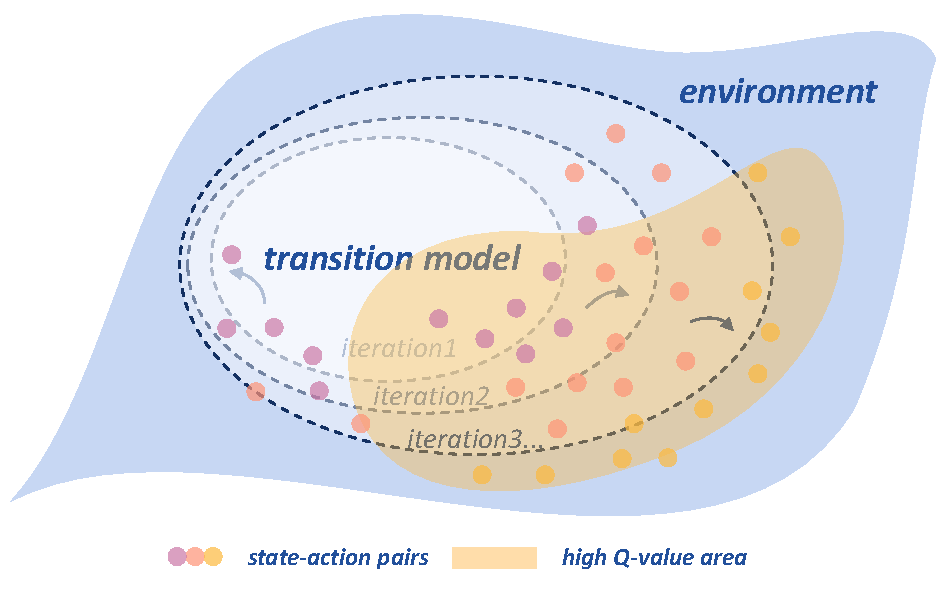
\includegraphics[width=0.6\textwidth]{figures/concept.pdf}
  \caption{基于定向探索模型的离线到在线强化学习算法框架。离线阶段利用不确定性惩罚保守更新策略；在线阶段利用不确定性引导定向探索，采集的样本用于更新转移模型和策略。}
  \label{Fig:Chap4_framework}
\end{figure}


\subsection{离线预训练阶段}\label{Sec4.2.1}

离线预训练阶段的目标是从静态数据集$\mathcal{D}_{off} = \{(s_i, a_i, s_i', r_i)\}_{i=1}^N$中学习环境动力学模型和初始策略。该阶段包含两个核心组件：集成转移模型的训练和基于不确定性惩罚的策略优化。

集成转移模型由$N$个独立训练的神经网络组成，每个网络$\hat{T}_\phi^i$以状态-动作对$(s,a)$为输入，输出下一状态和奖励的联合高斯分布：
\begin{equation}\label{Eq:Chap4_ensemble_model}
  \hat{T}_\phi^i(s', r|s, a) = \mathcal{N}(\mu_\phi^i(s, a), \Sigma_\phi^i(s, a)), \quad i = 1, \ldots, N
\end{equation}

其中$\mu_\phi^i(s, a) \in \mathbb{R}^{d_s + 1}$为预测均值向量，$\Sigma_\phi^i(s, a) \in \mathbb{R}^{(d_s+1) \times (d_s+1)}$为预测协方差矩阵，$d_s$为状态空间维度。各模型采用相同的网络结构但不同的随机初始化，通过最大化离线数据的对数似然独立训练：
\begin{equation}\label{Eq:Chap4_model_training}
  \mathcal{L}(\phi^i) = -\mathbb{E}_{(s,a,s',r) \sim \mathcal{D}_{off}}[\log \hat{T}_\phi^i(s', r|s, a)]
\end{equation}

集成模型的优势在于：一方面，多模型的平均预测可降低单一模型的偏差；另一方面，模型间预测的分歧度可用于量化认知不确定性，为后续的探索引导提供依据。

在策略优化方面，离线阶段采用基于不确定性惩罚的保守更新策略，遵循MOPO\cite{Yu2020MOPO}的框架。具体而言，定义离线阶段的不确定性估计为集成模型预测方差的最大值：
\begin{equation}\label{Eq:Chap4_offline_uncertainty}
  u_{off}(s, a) = \max_{i=1,\ldots,N} \|\Sigma_\phi^i(s, a)\|_F
\end{equation}

其中$\|\cdot\|_F$表示Frobenius范数。该度量捕捉了集成模型中最不确定的预测，反映状态-动作对$(s,a)$处环境动力学的偶然不确定性。基于此，定义不确定性惩罚奖励：
\begin{equation}\label{Eq:Chap4_penalized_reward}
  \tilde{r}(s, a) = \hat{r}(s, a) - \lambda_{off} \cdot u_{off}(s, a)
\end{equation}

其中$\hat{r}(s, a)$为转移模型预测的奖励均值，$\lambda_{off}$为惩罚系数。通过惩罚高不确定性区域的奖励，策略被约束在模型预测可靠的区域内优化，避免外推误差导致的性能退化。

策略优化采用Soft Actor-Critic（SAC）\cite{Haarnoja2018SAC}算法。SAC维护策略网络$\pi_\varphi$和两个Q值网络$Q_{\theta_1}, Q_{\theta_2}$，通过最大化带熵正则的期望回报优化策略：
\begin{equation}\label{Eq:Chap4_sac_objective}
  J(\varphi) = \mathbb{E}_{s \sim \mathcal{D}, a \sim \pi_\varphi}[Q_\theta(s, a) - \alpha \log \pi_\varphi(a|s)]
\end{equation}

其中$\alpha$为温度参数，控制探索与利用的平衡。Q值网络通过最小化时序差分误差更新：
\begin{equation}\label{Eq:Chap4_q_update}
  \mathcal{L}(\theta) = \mathbb{E}_{(s,a,\tilde{r},s') \sim \mathcal{D}}\left[(Q_\theta(s, a) - \tilde{r} - \gamma \mathbb{E}_{a' \sim \pi_\varphi}[\min_{j=1,2} Q_{\bar{\theta}_j}(s', a') - \alpha \log \pi_\varphi(a'|s')])^2\right]
\end{equation}

其中$\bar{\theta}$为目标网络参数。训练数据从离线数据集$\mathcal{D}_{off}$和模型生成数据集$\mathcal{D}_{model}$中按比例采样。模型生成数据通过从离线数据集中采样初始状态，利用当前策略与转移模型交互生成短期轨迹（rollout）获得。

离线预训练阶段完成后，获得初始策略$\pi_{off}$、集成转移模型$\{\hat{T}_\phi^i\}_{i=1}^N$以及Q值网络$Q_\theta$，为在线微调阶段提供基础。


\subsection{在线定向探索阶段}\label{Sec4.2.2}

在线微调阶段的核心目标是通过与真实环境的有限交互，采集高信息量样本以提升策略性能。与传统方法被动采样不同，本文提出的定向探索策略显式引导策略探索高不确定性且高价值的区域。

定向探索的核心思想是在策略优化目标中同时考虑不确定性和动作价值。具体而言，定义在线阶段的探索策略$\pi_\varphi$通过以下目标更新：
\begin{equation}\label{Eq:Chap4_exploration_objective}
  \nabla_\varphi J_\pi(\varphi) = \mathbb{E}_{(s,a) \sim \mathcal{D}_{on}}\left[\nabla_\varphi \log \pi_\varphi(a|s) \cdot (c \cdot u_{on}(s, a) + Q(s, a))\right]
\end{equation}

其中$u_{on}(s, a)$为在线阶段的不确定性估计（详见第\ref{Sec4.4}节），$Q(s, a)$为动作价值函数，$c$为平衡不确定性与价值的权重系数，$\mathcal{D}_{on}$为在线交互采集的数据集。

该目标函数的设计体现了定向探索的双重考量：

第一，不确定性项$u_{on}(s, a)$引导策略探索转移模型覆盖不足的区域。在这些高不确定性区域采集的样本对转移模型的改进贡献最大，可有效扩展模型的有效覆盖范围。从主动学习（Active Learning）的角度，这相当于选择模型最不确定的样本进行标注，是一种高效的数据收集策略。

第二，价值项$Q(s, a)$确保探索集中在高回报区域。单纯追求高不确定性可能导致策略探索与任务目标无关的状态-动作空间，造成在线交互资源的浪费。通过引入价值项，探索被引导至对策略优化有直接贡献的区域，实现探索效率与优化效果的平衡。

在线微调阶段的完整流程如下：

（1）与真实环境交互，使用当前探索策略$\pi_\varphi$采集轨迹数据，存入在线数据集$\mathcal{D}_{on}$。

（2）将在线数据与离线数据合并，更新集成转移模型$\{\hat{T}_\phi^i\}_{i=1}^N$。模型更新采用增量学习方式，在原有参数基础上继续训练，避免遗忘离线阶段学习的动力学知识。

（3）利用更新后的转移模型生成虚拟轨迹，结合真实数据更新Q值网络和策略网络。策略更新同时考虑标准SAC目标和定向探索目标。

（4）根据在线训练进度动态调整不确定性权重$c$（详见第\ref{Sec4.3.2}节），平衡探索与利用。

（5）重复上述步骤直至达到预设的在线交互预算或策略性能收敛。

通过上述迭代过程，转移模型逐步覆盖更广泛的状态-动作空间，策略在真实环境动力学下持续优化，最终实现高效的离线到在线迁移。


\section{不确定性估计与动态权重自适应}\label{Sec4.3}

不确定性估计是定向探索策略的核心组件。本节首先介绍离线和在线阶段采用的差异化不确定性估计方法，随后阐述动态权重自适应机制。


\subsection{双重不确定性估计}\label{Sec4.3.1}

如第二章所述，强化学习中的不确定性可分为偶然不确定性和认知不确定性两类。偶然不确定性源于环境固有的随机性，无法通过收集更多数据消除；认知不确定性源于模型对环境知识的缺乏，可通过在线探索逐步降低。在离线和在线两个阶段，两类不确定性的作用有所不同，因此本文采用差异化的不确定性估计方法。

在离线阶段，由于无法与真实环境交互，认知不确定性无法降低，因此主要关注偶然不确定性。偶然不确定性通过集成模型的预测方差估计：
\begin{equation}\label{Eq:Chap4_aleatoric_uncertainty}
  u_{off}(s, a) = \max_{i=1,\ldots,N} \|\Sigma_\phi^i(s, a)\|_F
\end{equation}

该度量反映环境动力学在状态-动作对$(s,a)$处的内在随机性。取集成模型中的最大方差是一种保守估计，确保在任一模型预测不确定时都施加惩罚。

在在线阶段，目标是主动探索高认知不确定性区域以补充转移模型。因此，除偶然不确定性外，还需捕捉认知不确定性。认知不确定性通过集成模型均值预测的分歧度估计：
\begin{equation}\label{Eq:Chap4_epistemic_uncertainty}
  \text{DisVar}(s, a) = \frac{1}{d}\sum_{j=1}^{d} \text{Var}_{i=1,\ldots,N}[\mu_{\phi,j}^i(s, a)]
\end{equation}

其中$d$为预测向量维度，$\mu_{\phi,j}^i(s, a)$为第$i$个模型预测均值的第$j$个分量，$\text{Var}_{i=1,\ldots,N}[\cdot]$表示在集成成员间计算方差。该度量的核心思想是：在数据充分覆盖的区域，各模型因接收到足够的监督信号而收敛至相近的预测，分歧度较低；在数据稀疏的区域，模型因初始化差异而产生显著不同的预测，分歧度较高。

在线阶段的不确定性估计综合两类不确定性：
\begin{equation}\label{Eq:Chap4_online_uncertainty}
  u_{on}(s, a) = \max_{i=1,\ldots,N} \|\Sigma_\phi^i(s, a)\|_F + \sqrt{\text{DisVar}(s, a)}
\end{equation}

第一项为偶然不确定性，第二项为认知不确定性的标准差形式。两项相加确保探索策略同时考虑环境的内在随机性和模型的知识缺乏，引导策略探索模型预测最不可靠的区域。


\subsection{动态权重自适应机制}\label{Sec4.3.2}

在定向探索目标（公式\ref{Eq:Chap4_exploration_objective}）中，权重系数$c$控制不确定性与价值的相对重要性。由于不同任务的状态空间和奖励尺度存在显著差异，$Q(s,a)$和$u_{on}(s,a)$的数值量级可能相差悬殊。为便于跨任务调节权重，首先对两项进行归一化处理。

具体而言，在离线阶段计算$\mathbb{E}_{(s,a) \sim \mathcal{D}_{off}}[Q(s,a)]$和$\mathbb{E}_{(s,a) \sim \mathcal{D}_{off}}[u(s,a)]$的均值和标准差。在线阶段，对计算得到的$Q(s,a)$和$u_{on}(s,a)$进行标准化：
\begin{equation}\label{Eq:Chap4_normalization}
  \bar{Q}(s,a) = \frac{Q(s,a) - \mu_Q}{\sigma_Q}, \quad \bar{u}_{on}(s,a) = \frac{u_{on}(s,a) - \mu_u}{\sigma_u}
\end{equation}

其中$\mu_Q, \sigma_Q$和$\mu_u, \sigma_u$分别为离线阶段统计得到的均值和标准差。归一化后，两项处于可比较的数值范围，权重$c$的调节更加直观。

此外，在在线微调过程中，不确定性与价值的相对重要性应随训练进度动态调整。在训练初期，模型覆盖范围有限，应优先探索高不确定性区域以扩展模型的有效范围；在训练后期，模型已较为完善，应转向利用已学习的知识优化策略，即更多关注高价值区域。

为实现上述动态平衡，本文采用Sigmoid函数调制权重$c$随策略更新步数$k$的衰减：
\begin{equation}\label{Eq:Chap4_dynamic_weight}
  c = c_0 \cdot \frac{1}{1 + e^{(k - k_0) \cdot \nu}}
\end{equation}

其中$c_0$为初始权重，$k_0$为衰减中心点，$\nu$为衰减速率。该函数具有以下特性：当$k < k_0$时，$c$接近$c_0$，策略重视不确定性引导的探索；当$k > k_0$时，$c$逐渐衰减至接近0，策略转向价值引导的利用；衰减过程平滑连续，避免策略行为的突变。

通过动态权重自适应机制，算法在训练初期充分探索以补充转移模型，在训练后期充分利用以优化策略性能，实现探索与利用的自适应平衡。


\section{理论分析}\label{Sec4.4}

本节从理论角度分析定向探索策略相比均匀采样的优势。核心结论是：在转移函数满足分段常数假设的条件下，基于不确定性引导的定向探索可实现更优的模型收敛速率。

在实际应用中，许多物理系统的动力学具有分段常数特性。例如，机器人控制任务中，不同操作模式（如空载与负载）对应不同的动力学参数；自动驾驶场景中，不同路面条件（如干燥与湿滑）导致车辆响应特性的显著差异。这些场景的转移函数可近似为在不同状态-动作区域内取不同常数值的分段常数函数。

\begin{defn}[分段常数函数]\label{Def:Chap4_piecewise_constant}
  设$\mathcal{X} \subset \mathbb{R}^d$为状态-动作空间的子集。函数$T: \mathcal{X} \rightarrow \mathbb{R}$称为分段常数函数，若存在$\mathcal{X}$的有限划分$\{R_1, \ldots, R_M\}$，使得$T$在每个区域$R_m$内取常数值$c_m$。记$\text{PC}(\beta, M)$为满足$\sum_{m=1}^{M}|\partial R_m|^\beta < \infty$的分段常数函数集合，其中$|\partial R_m|$表示区域$R_m$边界的测度，$\beta$为边界平滑性参数。
\end{defn}

基于上述定义，可建立定向探索策略的收敛速率下界。

\begin{thm}[定向探索的收敛速率]\label{Thm:Chap4_convergence}
  设转移函数$T \in \text{PC}(\beta, M)$为分段常数函数，$\hat{T}$为基于在线数据集$\mathcal{D}_{on}$学习得到的转移模型估计。若采样策略基于不确定性引导，即优先采样模型预测方差最大的状态-动作对，则模型估计误差的下界为：
  \begin{equation}\label{Eq:Chap4_convergence_bound}
    \inf_{\hat{T}} \sup_{T \in \text{PC}(\beta, M)} \mathbb{E}[\|\hat{T} - T\|^2] \geq c \cdot |\mathcal{D}_{on}|^{-\frac{1}{d-1}}
  \end{equation}
  其中$c > 0$为与区域复杂度相关的常数，$d$为状态-动作空间的内在维度，$|\mathcal{D}_{on}|$为在线数据集的样本数量。
\end{thm}

\begin{proof}
  该定理的证明基于主动学习理论中的经典结果\cite{Willett2005Faster}。核心思想是：对于分段常数函数，估计误差主要来源于函数不连续点（区域边界）附近的不确定性。基于不确定性引导的采样策略优先在这些边界区域采集样本，从而更高效地定位不连续点，降低估计误差。详细证明参见文献\cite{Willett2005Faster}中定理2的推导。
\end{proof}

作为对比，均匀采样策略的收敛速率下界为\cite{Korostelev1999Minimax}：
\begin{equation}\label{Eq:Chap4_uniform_bound}
  \inf_{\hat{T}} \sup_{T \in \text{PC}(\beta, M)} \mathbb{E}[\|\hat{T} - T\|^2] \geq c' \cdot |\mathcal{D}_{on}|^{-\frac{1}{d}}
\end{equation}

比较公式\ref{Eq:Chap4_convergence_bound}和公式\ref{Eq:Chap4_uniform_bound}，定向探索策略的收敛速率指数为$-\frac{1}{d-1}$，优于均匀采样的$-\frac{1}{d}$。这意味着在相同样本数量下，定向探索可实现更低的模型估计误差；或者，达到相同精度所需的样本数量更少。该理论结果为本文算法的样本效率优势提供了理论支撑。

需要指出的是，上述理论分析基于分段常数函数的假设，而实际环境的转移函数可能更为复杂。然而，分段常数函数可视为对复杂函数的局部近似，该理论结果仍具有指导意义：基于不确定性引导的定向探索在函数变化剧烈（对应高不确定性）的区域采集更多样本，有助于更精确地刻画转移函数的复杂结构。


\section{算法流程}\label{Sec4.5}

综合以上各节内容，本文提出的基于定向探索模型的离线到在线强化学习算法的完整流程如算法\ref{Alg:Chap4_DEM}所示。

\begin{algorithm}[htbp]
  \caption{基于定向探索模型的离线到在线强化学习算法}
  \label{Alg:Chap4_DEM}
  \begin{algorithmic}[1]
    \Require 离线数据集$\mathcal{D}_{off}$，集成模型数量$N$，离线训练轮数$E_{off}$，在线交互轮数$E_{on}$，初始探索权重$c_0$，衰减参数$k_0, \nu$，惩罚系数$\lambda_{off}$
    \Ensure 优化后的策略$\pi_\varphi$
    \State // 离线预训练阶段
    \State 初始化集成转移模型$\{\hat{T}_\phi^i\}_{i=1}^N$、策略网络$\pi_\varphi$、Q值网络$Q_{\theta_1}, Q_{\theta_2}$
    \For{$e = 1$ to $E_{off}$}
    \State 在$\mathcal{D}_{off}$上训练集成转移模型（公式\ref{Eq:Chap4_model_training}）
    \State 利用转移模型生成虚拟轨迹，存入$\mathcal{D}_{model}$
    \State 计算不确定性惩罚奖励$\tilde{r}$（公式\ref{Eq:Chap4_penalized_reward}）
    \State 从$\mathcal{D}_{off} \cup \mathcal{D}_{model}$采样，更新Q值网络和策略网络
    \EndFor
    \State 统计$\mathcal{D}_{off}$上$Q(s,a)$和$u(s,a)$的均值和标准差
    \State // 在线微调阶段
    \State 初始化在线数据集$\mathcal{D}_{on} \leftarrow \emptyset$
    \For{$e = 1$ to $E_{on}$}
    \State 使用策略$\pi_\varphi$与真实环境交互，采集轨迹数据加入$\mathcal{D}_{on}$
    \State 合并$\mathcal{D}_{off}$和$\mathcal{D}_{on}$，更新集成转移模型
    \State 计算在线不确定性$u_{on}(s,a)$（公式\ref{Eq:Chap4_online_uncertainty}）
    \State 更新动态权重$c$（公式\ref{Eq:Chap4_dynamic_weight}）
    \State 利用定向探索目标更新策略（公式\ref{Eq:Chap4_exploration_objective}）
    \State 更新Q值网络
    \EndFor
    \State \Return 策略$\pi_\varphi$
  \end{algorithmic}
\end{algorithm}

算法的时间复杂度主要由以下部分组成：（1）集成模型训练，复杂度为$O(N \cdot |\mathcal{D}| \cdot d_{model})$，其中$d_{model}$为模型参数量；（2）不确定性估计，复杂度为$O(N \cdot d)$，其中$d$为预测向量维度；（3）策略和Q值网络更新，与标准SAC相同。由于集成模型可并行训练，实际计算开销与单模型方法相当。

算法的空间复杂度主要由集成模型参数和经验回放池占用。集成模型的参数量为$O(N \cdot d_{model})$，经验回放池的存储需求与数据集大小成正比。在实际实现中，$N$通常取5-7，不会显著增加存储开销。


\section{实验验证}\label{Sec4.7}

本节通过在D4RL基准测试集上的实验验证本文算法的有效性。实验设计旨在回答以下问题：（1）本文算法与现有离线到在线强化学习方法及基于模型的离线强化学习方法相比表现如何？（2）基于不确定性引导的定向探索是否确实聚焦于高不确定性、高价值区域？（3）动态权重自适应机制对最终性能的贡献如何？


\subsection{实验设置}\label{Sec4.7.1}

本节介绍实验所采用的数据集、实现细节和基线方法。

在数据集选择方面，本文在D4RL基准测试集\cite{Fu2020D4RL}上评估算法性能。D4RL是基于MuJoCo物理仿真器\cite{Todorov2012MuJoCo}构建的离线强化学习标准评测平台，包含多种环境和数据集类型。本文选取三种连续控制环境（halfcheetah、hopper、walker2d）和三种数据集类型（medium、medium-replay、medium-expert），共计9个问题设置。所有数据集均采用v2版本，具体组成如下：（1）medium数据集包含由提前终止的SAC策略生成的转移样本，代表中等质量的离线数据；（2）medium-replay数据集由训练medium策略过程中的经验回放池组成，包含从随机策略到中等策略的完整训练轨迹；（3）medium-expert数据集混合了次优策略和专家策略的数据，代表高质量但分布不均匀的离线数据。

在实验实现方面，本文遵循SAC\cite{Haarnoja2018SAC}和MOPO\cite{Yu2020MOPO}的基本超参数设置。需要调整的超参数主要包括模型生成轨迹的长度$h$和惩罚系数$\lambda_{off}$。所有任务均在3个随机种子上运行。在线交互阶段，每轮交互采集50k步样本，权重调整速率$\nu$设为0.001，衰减中心点$k_0$设为5000。为保证公平性和一致性，策略训练总步数设为1M步，每1k步评估一次策略性能。

在基线方法方面，本文与以下算法进行对比：离线到在线强化学习算法AWAC\cite{Nair2020AWAC}；基于模型的离线强化学习算法MOPO\cite{Yu2020MOPO}、COMBO\cite{Yu2021COMBO}和MOREL\cite{Kidambi2020MOReL}；经典离线强化学习算法CQL\cite{Kumar2020CQL}和TD3+BC\cite{Fujimoto2021TD3BC}。由于本文算法建立在MOPO基础上并增加在线微调过程，与MOPO的对比可视为消融研究。所有基线方法的结果均引用自原始论文。


\subsection{实验结果}\label{Sec4.7.2}

表\ref{Tab:Chap4_Performance}展示了本文算法与基线方法在D4RL基准测试集上的性能对比。实验结果报告为最后10次评估的平均归一化得分，$\pm$表示3个随机种子的标准差。得分采用D4RL标准归一化程序\cite{Fu2020D4RL}，归一化至0到100的范围，其中0分对应随机策略，100分对应专家策略。

\begin{table}[htbp]
  \centering
  \caption{D4RL基准测试集上的性能对比}
  \label{Tab:Chap4_Performance}
  \resizebox{\textwidth}{!}{
    \begin{tabular}{llrrrrrrr}
      \toprule
      数据集类型         & 环境          & 本文算法                     & MOPO & COMBO & AWAC  & MOREL & CQL   & TD3+BC           \\
      \midrule
      medium        & halfcheetah & $\mathbf{70.5 \pm 4.2}$  & 42.3 & 54.2  & 41.1  & 42.1  & 44.4  & 42.8             \\
                    & hopper      & $65.5 \pm 10.9$          & 28.0 & 97.2  & 91.0  & 95.4  & 86.6  & $\mathbf{99.5}$  \\
                    & walker2d    & $\mathbf{86.6 \pm 0.5}$  & 17.8 & 81.9  & 79.1  & 77.8  & 74.5  & 79.7             \\
      \midrule
      medium-replay & halfcheetah & $\mathbf{73.1 \pm 0.4}$  & 53.1 & 55.1  & -     & 40.2  & 46.2  & 43.3             \\
                    & hopper      & $\mathbf{96.1 \pm 5.9}$  & 67.5 & 89.5  & -     & 93.6  & 48.6  & 31.4             \\
                    & walker2d    & $\mathbf{82.6 \pm 0.3}$  & 39.0 & 56.0  & -     & 49.8  & 32.6  & 25.2             \\
      \midrule
      medium-expert & halfcheetah & $75.4 \pm 13.3$          & 63.3 & 90.0  & 41.0  & 53.3  & 62.4  & $\mathbf{97.9}$  \\
                    & hopper      & $102.2 \pm 0.8$          & 23.7 & 111.1 & 111.9 & 108.7 & 111.0 & $\mathbf{112.2}$ \\
                    & walker2d    & $\mathbf{111.4 \pm 0.4}$ & 44.6 & 103.3 & 78.3  & 95.6  & 98.7  & 101.1            \\
      \bottomrule
    \end{tabular}
  }
\end{table}

从表\ref{Tab:Chap4_Performance}可以看出，本文算法在多数任务上取得了优异的性能表现。在medium-replay数据集的全部三个环境中，本文算法均取得最高得分，显著优于所有基线方法。这一结果表明，当离线数据质量参差不齐时，本文的定向探索策略能够有效识别并补充高价值区域的样本，显著提升策略性能。

值得注意的是，本文算法在所有9个问题设置上均优于MOPO算法，验证了在线微调框架的有效性。考虑到本文仅使用50k步的在线交互量，远低于传统离线到在线强化学习算法所需的200k步以上，这一结果尤为突出。

然而，本文算法在medium-expert数据集上的表现相对较弱。分析其原因在于：medium-expert数据集的离线数据高度集中在高奖励区域，导致期望奖励高但不确定性低。这种数据分布限制了在线交互阶段采集的数据多样性和质量，进而约束了算法的提升空间。相比之下，基于行为克隆的强化学习方法（如TD3+BC）在高质量数据集上表现优异，这为后续改进提供了思路：引入行为克隆损失项可能有助于提升算法在此类环境中的性能。


\subsection{模型覆盖范围的可视化验证}\label{Sec4.7.3}

为验证基于不确定性引导的定向探索是否确实聚焦于高期望回报和高不确定性区域，本节进行可视化实验分析。具体而言，选取三种不同类型的数据集进行可视化：hopper-medium、hopper-medium-replay和hopper-medium-expert。

实验过程如下：首先，从离线数据集中采样2000个转移样本$(s, a, s', r)$；然后，将离线状态$s$输入转移模型，获得模型预测的转移样本$(s, a_T, s'_T, r_T)$；接着，使用t-SNE算法\cite{vanderMaaten2008tSNE}将$\{s'\}$和$\{s'_T\}$投影至二维平面；最后，绘制$\{s'_T\}$的散点图，使用离线策略的Q值网络估计状态-动作对$(s, a_T)$的期望回报，并将Q值映射为散点颜色。同时，显示离线状态$\{s'\}$的核密度估计作为参照。可视化结果如图\ref{Fig:Chap4_tsne}所示。

\begin{figure}[htbp]
  \centering
  
\includegraphics[width=1\textwidth]{figures/tsne.pdf}
  \caption{模型预测状态与离线数据的对比。将模型预测状态和离线状态数据密度在三种不同离线数据集上进行可视化。散点表示模型的数据分布，预测Q值经归一化后作为散点的颜色。}
  \label{Fig:Chap4_tsne}
\end{figure}

从图\ref{Fig:Chap4_tsne}可以观察到，模型预测的状态主要分布在低密度的边缘区域，且散点大多呈现红色，表明这些区域具有高不确定性和高期望回报。这一现象表明，在策略引导下，模型确实更多地关注高不确定性且高动作价值的区域。

对比三个子图可以发现：在hopper-medium-replay环境中，散点分布较为分散，表明在线交互实现了充分的探索，补充了更多分布外数据；在hopper-medium-expert环境中，散点分布更为集中，这是因为专家数据的高质量和低方差使得在线交互难以通过探索采集到更高动作价值的数据，导致补充的数据质量可能不及离线数据集中的专家数据，模型更新不够充分。这一观察结果进一步印证了本文算法更适用于数据分布均匀的环境，而在高质量数据集上的适用性有限。


\subsection{动态权重自适应的消融实验}\label{Sec4.7.4}

为验证动态权重自适应机制的有效性，本节设计消融实验，将完整算法与移除动态权重自适应的变体（记为DEM-s）进行对比。DEM-s中，不确定性权重参数$c$固定为初始值$c_0$，不随在线交互步数增加而衰减。其余超参数与主实验保持一致。

\begin{table}[htbp]
  \centering
  \caption{动态权重自适应的消融实验结果}
  \label{Tab:Chap4_ablation}
  \begin{tabular}{llrr}
    \toprule
    数据集类型         & 环境          & 本文算法            & 无动态权重            \\
    \midrule
    medium        & halfcheetah & $\mathbf{70.5}$ & $64.7$           \\
                  & hopper      & $\mathbf{65.5}$ & $53.0$           \\
                  & walker2d    & $\mathbf{86.6}$ & $86.2$           \\
    \midrule
    medium-replay & halfcheetah & $\mathbf{73.1}$ & $72.6$           \\
                  & hopper      & $\mathbf{96.1}$ & $90.2$           \\
                  & walker2d    & $\mathbf{82.6}$ & $82.1$           \\
    \midrule
    medium-expert & halfcheetah & $\mathbf{75.4}$ & $36.1$           \\
                  & hopper      & $102.2$         & $102.2$          \\
                  & walker2d    & $111.4$         & $\mathbf{112.0}$ \\
    \bottomrule
  \end{tabular}
\end{table}

表\ref{Tab:Chap4_ablation}展示了消融实验结果。完整算法在几乎所有任务上均取得更优性能，尤其在hopper-medium和halfcheetah-medium-expert任务上提升显著：完整算法分别取得65.5和75.4的得分，而无动态权重变体仅为53.0和36.1。然而，在walker2d-medium-expert任务上，完整算法略低于无动态权重变体，推测这与该任务高度结构化的专家数据有关，早期探索阶段可能对策略产生轻微干扰。

上述结果表明，动态权重自适应机制在平衡探索与利用方面发挥了关键作用。在交互初期，较高的不确定性权重鼓励探索，使策略覆盖更广泛的状态-动作空间；随着交互推进，权重逐渐降低，使算法聚焦于高奖励区域并稳定策略性能。这种自适应机制使算法能够根据训练进度动态调整探索-利用平衡，优于固定权重的静态策略。


\section{本章小结}\label{Sec4.8}

本章详细介绍了基于定向探索模型的离线到在线强化学习算法。首先分析了现有方法在保守性与灵活性、不确定性利用、在线交互成本等方面的局限，阐明了将不确定性从惩罚信号转变为探索引导信号的核心思想。随后系统阐述了算法的两阶段框架：离线阶段通过集成模型和不确定性惩罚进行保守策略优化；在线阶段通过定向探索目标引导策略探索高不确定性且高价值的区域，以最少的在线交互实现高效微调。

在技术实现层面，本章介绍了双重不确定性估计方法，区分偶然不确定性和认知不确定性在不同阶段的作用；提出了动态权重自适应机制，通过Sigmoid函数实现探索与利用的平滑过渡。在理论分析层面，证明了在分段常数函数假设下，定向探索策略相比均匀采样具有更优的收敛速率，为算法的样本效率优势提供了理论支撑。

在实验验证层面，本章在D4RL基准测试集的9个问题设置上进行了系统评估。实验结果表明：（1）本文算法在medium-replay数据集上显著优于所有基线方法，在所有任务上均优于MOPO；（2）通过t-SNE可视化验证了定向探索确实聚焦于高不确定性、高价值区域；（3）消融实验证明了动态权重自适应机制对最终性能的积极贡献。实验同时揭示了算法在high-quality数据集上的局限性，为后续改进指明了方向。

\chapter{总结与展望}\label{Chap:chap5}

\section{本文工作总结}\label{Sec5.1}

离线强化学习通过从预先收集的静态数据集中学习策略，避免了在线交互的高昂成本与安全风险，在医疗诊断、自动驾驶、机器人控制、金融决策等实际应用场景中具有重要价值。然而，离线数据集的有限覆盖范围导致的分布偏移问题是制约该技术发展的核心挑战：当智能体的策略访问离线数据未覆盖的状态-动作对时，价值函数的估计将产生外推误差，导致策略性能显著低于预期。本文围绕离线强化学习中的不确定性估计与探索策略展开系统研究，针对纯离线设定和离线到在线设定分别提出了两种互补的算法方案，取得了以下研究成果：

第一，提出基于自适应不确定性度量的离线强化学习算法。针对现有基于模型方法仅考虑状态转移不确定性、采用静态惩罚系数的局限，本文从两个维度进行改进：在不确定性度量层面，引入累积状态不确定性的概念，通过递推公式$u(s') = \omega \cdot u(s) + \log(\Sigma_\theta(s, a) + 1)$综合考虑从初始状态到当前状态的历史不确定性累积效应，使智能体能够更全面地评估序列决策中的风险累积；在惩罚调节层面，设计基于Sigmoid函数的自适应动态权重机制$\lambda_k = \lambda_0 / (1 + e^{K_0 - k})$，根据策略优化进程动态调节不确定性惩罚强度，在训练初期降低惩罚以鼓励探索搜索策略空间，在策略逐渐收敛时增加惩罚以保持保守性确保策略稳定。理论分析证明了累积不确定性沿轨迹的单调不减性质和不确定性预测网络的泛化能力，以及自适应权重相比固定权重在探索-保守平衡方面的优势。在D4RL MuJoCo基准测试集上的实验表明，该方法在9个任务中的6个取得最优或接近最优性能，特别是在数据质量较差的随机数据集上相比MOPO取得了显著提升（halfcheetah任务从35.4提升至37.2，hopper任务从11.7提升至17.6），在hopper-medium任务上提升幅度达44.4个百分点。

第二，提出基于定向探索模型的离线到在线强化学习算法。针对现有离线到在线方法保守性与灵活性矛盾、不确定性利用不充分、在线交互成本高等问题，本文提出将不确定性信息从“惩罚信号”转变为“探索引导信号”的核心思想。在离线阶段，通过集成模型和不确定性惩罚进行保守策略优化，确保策略在模型预测可靠的区域内更新；在在线阶段，通过定向探索目标$\nabla_\varphi J_\pi(\varphi) = \mathbb{E}[\nabla_\varphi \log \pi_\varphi(a|s) \cdot (c \cdot u_{on}(s, a) + Q(s, a))]$显式引导策略探索高不确定性（转移模型覆盖之外）且高动作价值（接近任务目标）的区域。在技术层面，提出双重不确定性估计方法区分偶然不确定性和认知不确定性在不同阶段的作用：离线阶段使用集成模型的预测方差估计偶然不确定性以实现保守性，在线阶段同时使用预测方差和集成分歧度估计两类不确定性以引导探索。设计动态权重自适应机制$c = c_0 / (1 + e^{(k - k_0) \cdot \nu})$实现探索与利用的平滑过渡，在交互初期注重不确定性引导的探索，在交互后期转向价值引导的利用。理论分析证明了在分段常数函数假设下，定向探索策略相比均匀采样具有更优的收敛速率（指数从$-1/d$改善至$-1/(d-1)$）。实验结果表明，该方法仅需50k步在线交互即可在medium-replay数据集上显著优于所有基线方法，在所有9个任务上均优于MOPO，通过t-SNE可视化验证了定向探索确实聚焦于高不确定性、高价值区域。

两种方法形成递进关系：首先，本文提出基于自适应不确定性度量的离线强化学习算法，解决纯离线设定下的保守策略优化问题；其次，引入在线微调阶段的定向探索模型，将“被动惩罚分布外”转变为“主动探索分布外”。两种方法共同构成了从纯离线到离线在线联合优化的完整技术方案。


\section{进一步研究方向}\label{Sec5.2}

尽管本文提出的方法在实验中取得了良好效果，但仍存在一定局限性，有待进一步研究改进。在算法效率方面，本文方法需要额外训练不确定性预测网络，增加了模型复杂度和训练开销，未来可探索更轻量级的不确定性估计方法，如基于梯度信息的在线估计、基于核方法的非参数估计、或利用神经网络中间层特征的即时估计，在保持估计精度的同时降低计算成本；在理论基础方面，本文采用Sigmoid函数实现惩罚权重的平滑过渡，但最优的过渡曲线可能与任务特性相关，未来可研究基于元学习或贝叶斯优化的自动权重调节方法，从数据中自适应学习最优的探索-保守平衡策略。

在算法适用性方面，实验表明本文方法在medium-expert等高质量数据集上的提升有限，这是因为专家数据的高集中度限制了定向探索的空间，未来可引入行为克隆损失项或设计自适应的探索门控机制，使算法能够根据离线数据质量自动调节探索强度——在低质量数据上加强探索以突破次优策略的局限，在高质量数据上减少探索以避免干扰专家知识；在分布外检测方面，本文方法主要基于集成模型的不确定性估计，未来可探索将表征学习与不确定性估计相结合的方法，通过学习状态-动作空间的紧致表征，利用表征空间的几何结构（如到数据中心的距离）实现更精确的分布外检测。

在应用拓展方面，本文方法针对单一任务设计，在多任务学习或任务迁移场景中可能需要额外的适配机制，未来可研究跨任务的不确定性共享与迁移方法，使模型能够利用相关任务的经验加速学习；在实际应用中的安全约束方面，医疗、自动驾驶等高风险场景除了性能优化外还需满足安全约束，未来可将本文的不确定性估计方法与约束强化学习相结合，在保证安全边界的前提下实现策略优化，例如将不确定性估计融入安全约束的构建，在高不确定性区域施加更严格的安全裕度。综合各方面分析，离线强化学习作为连接历史数据与智能决策的重要桥梁，具有广阔的应用前景。本文的研究为不确定性驱动的离线策略优化提供了新的思路，特别是将不确定性从被动规避的风险转化为主动利用的探索信号，为该领域的后续研究开辟了新的方向。

\chapter{总结与展望}\label{Chap:chap6}

\section{本文工作总结}\label{Sec6.1}
《正文》********************



\section{进一步研究方向}\label{Sec6.2}
《正文》********************







% 参考文献，五号字，使用 BibTeX，包含参考文献文件.bib
\bibliography{reference/Ref_Article,reference/Ref_Conference,reference/Ref_Book}




%%%%%%%%%%%%后置部分%%%%%%%%%%%%
% 附录(章节编号重新计算，使用字母进行编号)
\appendix


%(其后部分无编号)
\backmatter

% 程序清单
%%==================================================
%% resume.tex for BIT Master Thesis
%% modified by yang yating
%% version: 0.1
%% last update: Dec 25th, 2016
%%==================================================

\begin{ProgramList}

第\ref{Chap:chap3}章 QAM系统CMA算法程序（QAM programme文件夹）

mainQAM\_MSE\_CMAvsCADAMA：QAM系统，画MSE曲线主函数

mainQAM\_SER\_CMAvsCADAMA：QAM系统，画SER曲线主函数

mainDQAM\_SER\_PhaseRotate：差分QAM系统，相位旋转下，画SER曲线主函数

mainDQAM\_SER\_Doppler：差分QAM系统，多普勒频移下，画SER曲线主函数

mainDQAM\_SER\_SNR：差分QAM系统，不同SNR下，画SER曲线主函数
\\









第\ref{Chap:chap4}章 QPSK系统CMA算法程序（PSK programme文件夹）

mainDPSK\_SER\_PhaseRotate：差分PSK系统，相位旋转下，画SER曲线主函数

mainDPSK\_SER\_Doppler：差分PSK系统，多普勒频移下，画SER曲线主函数

mainDPSK\_SER\_SNR：差分PSK系统，不同SNR下，画SER曲线主函数

FunQPSK：QPSK编码子函数

FunDeQPSK\_b：QPSK解码子函数(输出为比特)
\\












第\ref{Chap:chap5}章 CMA频域均衡系统程序（FDE programme文件夹）

main\_CMAFDE：CMA频域均衡主函数

FunCAZACSeGen：产生CAZAC序列子函数

Fun8PSK：8PSK调制子函数

FunDe8PSK\_s：8PSK解调 输出符号子函数

FunQPSK1：QPSK调制幅度为1子函数

FunDeQPSK1\_s：QPSK解调 输出符号 幅度为1子函数

FunSDCMA22f：频域均衡(2 2)SDCMA算法子函数


\end{ProgramList}

% 发表文章目录
\begin{publications}{0000}
    %这里与参考文献一样，按照“GB/T 7714”格式 复制出论文引用，后面加上（检索信息），SCI论文需要写上几区。

    \item [{[1]}] 张伯雷, 刘哲闰. 基于自适应不确定性度量的离线强化学习算法[J]. 南京邮电大学学报(自然科学版), 2024, 44(4):98-104. (中英文对照：Adaptive Uncertainty Quantification for Model-based Offline Reinforcement Learning, doi:10.14132/j.cnki.1673-5439.2024.04.009)

    %本人名字可用\bf{}加粗

\end{publications}











% 发表专利目录
\begin{patent}{00}

    \item [{[1]}]  作者一，作者二，作者三. 专利名称，专利申请号，专利申请日期，专利授权日期；
    
    \item [{[2]}]  张三，李四. 一种面向代理的安全传输方法，2007062.5，2016.1,2017.10；
    
    \item [{[3]}]  张三. 一种实用的网络路由方法，200845610.5，2017,1,2018.1。

\end{patent}


% 参与项目目录
\begin{publicationsProjects}{000}

    \item [{[1]}]  国家自然科学基金青年项目，基于多智能体强化学习的复杂社会困境合作机制研究(62202238)，2023.01-2025.12，负责人，张伯雷。

\end{publicationsProjects}


% % 致谢
%\begin{thanks}
  论文写到这里的时候，学科楼前的海棠花快要落完了。风一吹，花瓣像轻轻的标点，落在台阶上、走廊里，也落在这一段时光的末尾。春天走到尾声，我的求学生涯也慢慢收拢成一个句号。若要用一句话概括此刻的心情，我最想说的不是“完成了”，而是“谢谢”。

  首先要感谢我的导师张伯雷老师。谢谢您在我最迷茫、最容易怀疑自己的时候，仍愿意把时间分给我，把问题重新摆到光亮处：该从哪里下手、为什么这样做、怎样把一件事做得更扎实。您对研究的严谨与克制、对细节的敏感，以及在关键节点上不动声色的托举，构成了我这段经历里最可靠的坐标。

  感谢课题组的同学们。许多想法并不是在某个瞬间“突然拥有”，而是在一次次讨论、争辩与推演里逐渐成形：被追问到语塞的那几分钟、在白板前反复擦写的那些式子、把一组不理想的结果拆开重看的耐心。谢谢你们在我卡住的时候一起把思路捋直，在我实验崩掉的时候陪我把错误找出来，也在我有一点点进展的时候，愿意认真听我把它讲完。

  感谢陪我一起吃饭散步的朋友。你们未必关心我用的是哪一种算法，却会关心我有没有好好吃饭、能不能按时睡觉；你们不一定看得懂图表和符号，却愿意在我最焦虑的时候陪我把情绪放回原位。那些看似与论文无关的温柔与照拂，恰恰让我有力气继续写下去。

  感谢美丽的南京邮电大学。谢谢这几年里一路相伴的花花草草：雨后更亮的叶子、傍晚被夕阳照得发暖的树影、以及每一个在图书馆和实验室之间奔波的清晨与深夜。也谢谢校园里那些可爱的小猫——它们不懂我的焦虑与截止日期，却用一次擦肩、一次停留，让我在最紧绷的时候重新想起呼吸和松弛。很多时候，生活里这些微小而确切的美，恰好把我从无数次“差一点坚持不下去”里拉回来。

  最后，也想谢谢那个在反复修改、不断推翻重来的过程中没有放弃的自己。愿这段经历留下的，不止是一份阶段性的成果，更是一种在迷雾里继续前行的勇气与能力。

\end{thanks}


\end{document} 